\documentclass[UTF8, mathserif]{ctexbeamer}

\usetheme{Boadilla}

% Chinese
% \setCJKmainfont[BoldFont={SimHei},ItalicFont={KaiTi}]{KaiTi}

% Title
\title{数学建模与Matlab}
\subtitle{第一章 对变化进行建模}
\author{韩建伟}
\institute{
  计信学院\\
  \texttt{mm@hanjianwei.com}
}
\date{2017/09/22}

\begin{document}

% Title page
\begin{frame}[plain]
  \titlepage{}
\end{frame}

\begin{frame}{课程介绍}

\begin{description}
\item[内容] 数学建模 + Matlab
\item[教材] 数学建模(原书第5版), Frank R.Giordano, Willam P.Fox, Steven B.Horton, 叶其孝 / 姜启源译, 机械工业出版社
\item[参考] 数学模型(第四版), 姜启源 / 谢金星 / 叶俊, 高等教育出版社\\
  数学建模, 杨启帆 / 谈之奕 / 何勇, 浙江大学出版社\\
  精通MATLAB R2011a, 张志涌, 北京航天航空大学出版社
\item[网站] http://zjsu.github.io/mm
\end{description}
  
\end{frame}

\begin{frame}{课程安排}
  \begin{description}
  \item[时间] 15周 = 12课堂 + 2实验 + 1假期
  \item[考试] 成绩 = 平时 $\times$ 30\%+ 期末(闭卷) $\times$ 70\%
  \item[作业] 作业 = 小作业 + 大作业(2-3人一个团队)
  \end{description}
\end{frame}

\begin{frame}{课程概要}
  \begin{center}
    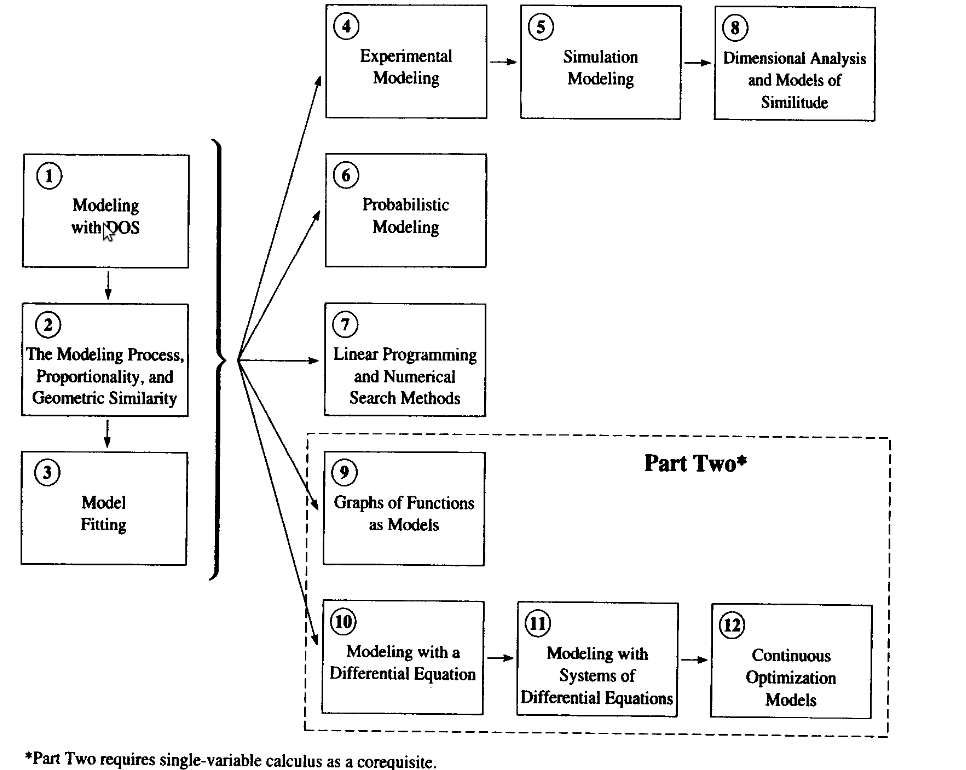
\includegraphics[height=.8\textheight{}]{book-overview.png}
  \end{center}
\end{frame}

\begin{frame}{简介}

数学模型是对现实世界现象的理想化表示而非完全精确的表示.

\begin{itemize}
\item 预测变化
\item 对现实世界进行简化
  \begin{center}
    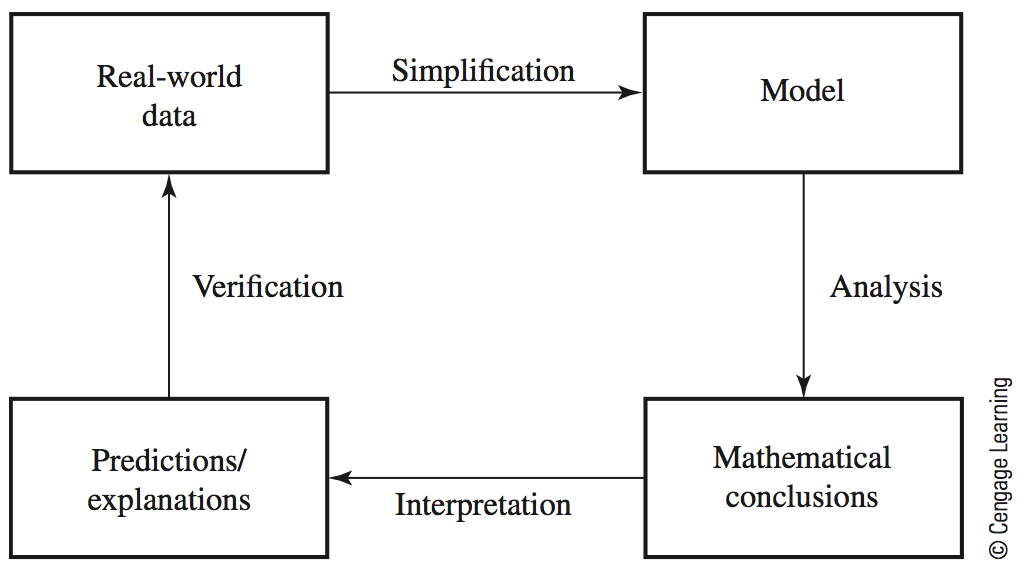
\includegraphics[width=.5\textwidth{}]{model.png}
  \end{center}
  例如: 比例性.
\end{itemize}
  
\end{frame}

\begin{frame}{弹簧系统}
  \begin{center}
    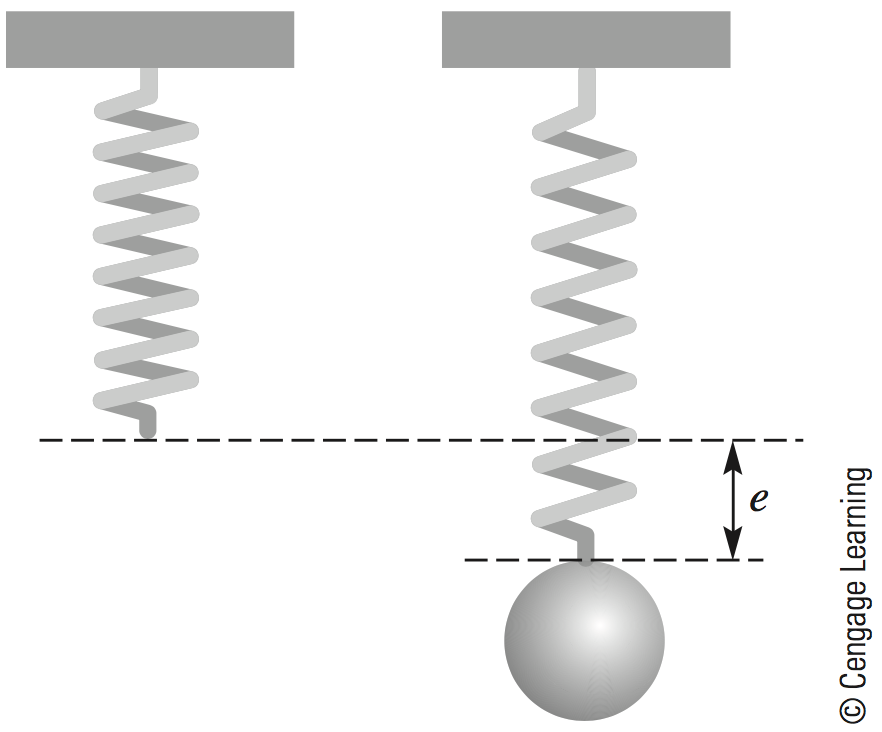
\includegraphics[width=.4\textwidth{}]{spring.png}
    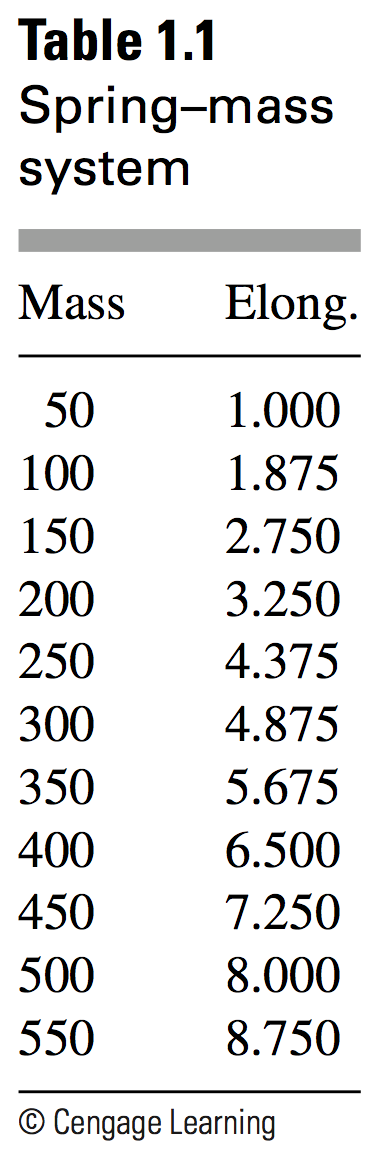
\includegraphics[width=.15\textwidth{}]{spring-table.png}
  \end{center}
  \[
  slope = \frac{4.875 - 3.25}{300 - 200} = 0.01625
  \]
\end{frame}

\begin{frame}{验证弹簧系统}
  \[
  e = 0.0163
  \]

  \begin{center}
    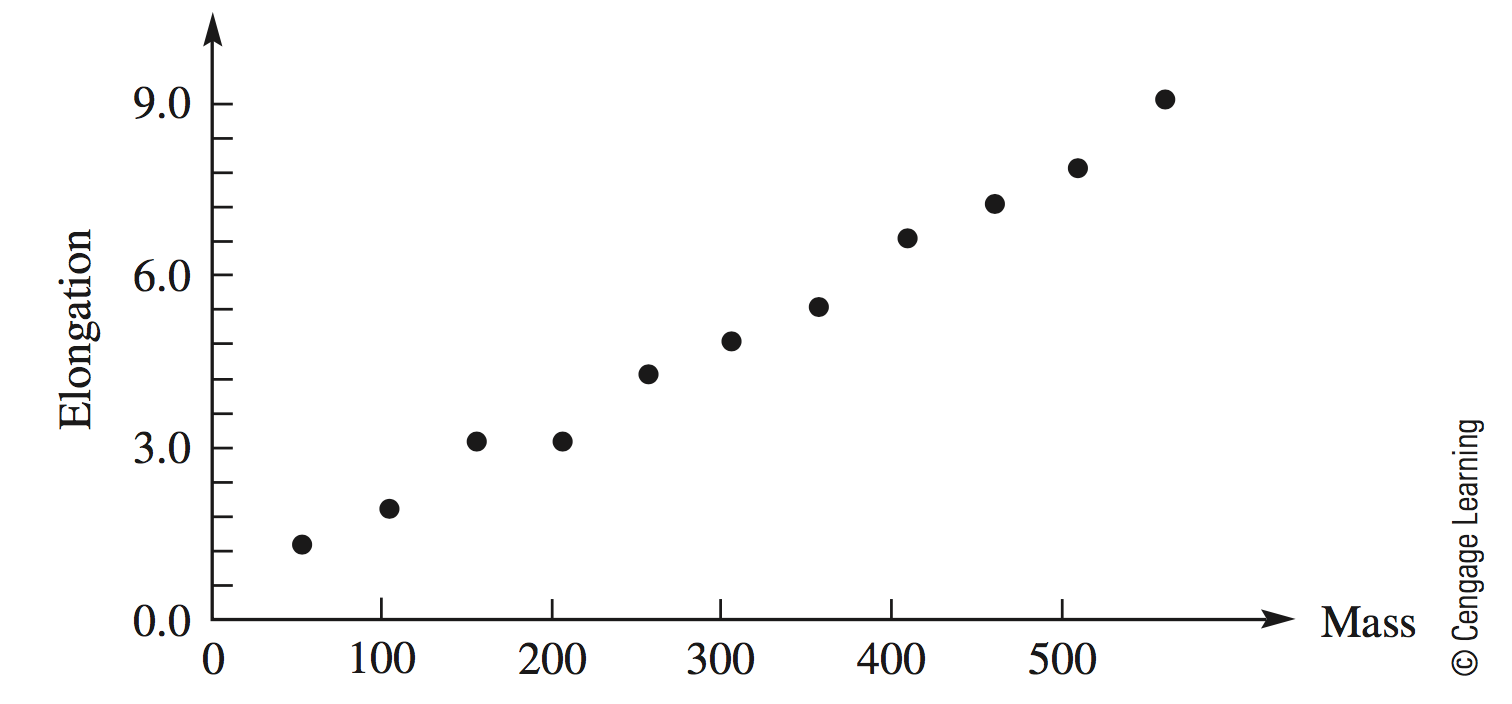
\includegraphics[width=.4\textwidth{}]{spring-plot.png}
    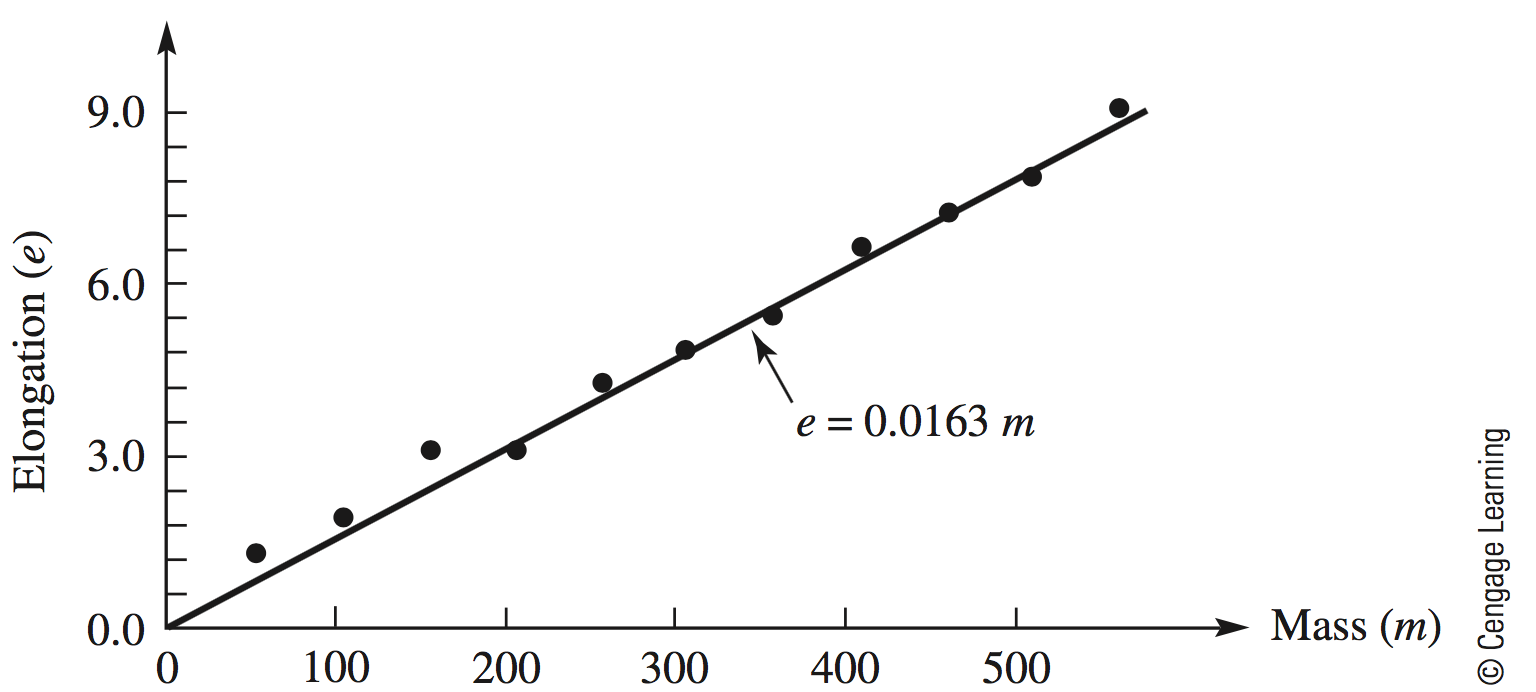
\includegraphics[width=.4\textwidth{}]{spring-slope.png}
  \end{center}
\end{frame}

\begin{frame}{对变化进行建模}
  未来值 = 现在值 + 变化

  变化 = 未来值 - 现在值

  \begin{description}
  \item[离散时间] 差分方程(difference equation)
  \item[连续时间] 微分方程(第11章)
  \end{description}
  
\end{frame}

\begin{frame}{差分方程}

  \begin{definition}
    对于数列$A = {a_0, a_1, a_2, a_3, ...}$, 其一阶差分定义为:
    \[
    \Delta a_0 = a_1 - a_0
    \]\\[-25pt]
    \[
    \Delta a_1 = a_2 - a_1
    \]\\[-25pt]
    \[
    \Delta a_2 = a_3 - a_2
    \]\\[-25pt]
    \[
    \Delta a_3 = a_4 - a_3
    \]
    对于每个正整数$n$, 第$n$个一阶差分为:
    \[
    \Delta a_n = a_{n+1} - a_n
    \]
  \end{definition}
\end{frame}

\begin{frame}{差分方程}
  \begin{center}
    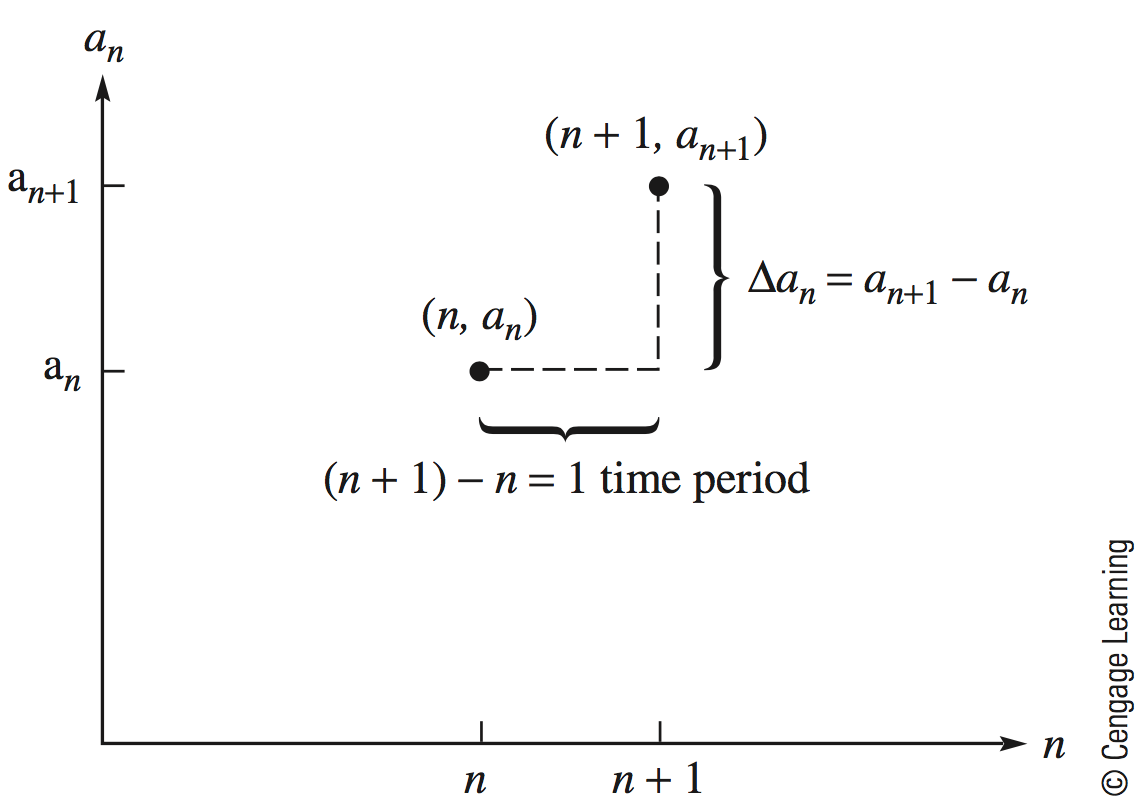
\includegraphics[width=.6\textwidth{}]{difference.png}
  \end{center}
\end{frame}

\begin{frame}{储蓄问题}
考虑本金1000美元, 月利息1\%的储蓄问题$A = (1000, 1010, 1020.10, 1030.30, ...)$.
\begin{block}{}
    \[
    \Delta a_0 = a_1 - a_0 = 1010.0 - 1000.0 = 10.0
    \]\\[-25pt]
    \[
    \Delta a_1 = a_2 - a_1 = 1020.1 - 1010.0 = 10.1
    \]\\[-25pt]
    \[
    \Delta a_2 = a_3 - a_2 = 1030.3 - 1020.1 = 10.2
    \]
\end{block}

\[
\Delta a_n = a_{n+1} - a_n = 0.01a_n
\]\\[-25pt]
\[
a_{n+1} = a_n + 0.01a_n = 1.01a_n, n = 0, 1, 2, 3
\]\\[-25pt]
\[
a_0 = 1000
\]
  如果每月取出50美元...
\[
\Delta a_n = a_{n+1} - a_n = 0.01a_n - 50
\]

\end{frame}

\begin{frame}{如何找出变化}

在多数情况下, 很难象上述例子那样精确表述, 因此我们通过如下步骤找出变化:

\begin{enumerate}
\item 画出变化
\item 观察变化规律
\item 用数学术语描述变化
\end{enumerate}

变化 = $\Delta a_n$ = 某个函数$f$

对于离散情况:

变化 = $\Delta a_n$ = $a_{n+1} - a_n$ = $f$(序列中的项, 外部项)
\end{frame}

\begin{frame}{按揭买房}
六年前按揭20年买了一套80000美元的房子, 月供880.87美元并付每月1\%的利息. 问现在还欠银行多少?
\[
\Delta b_n = b_{n+1} - b_n = 0.01b_n - 880.87
\]

求解下列方程即可:

\begin{block}{}
\[
b_{n+1} = b_n + 0.01b_n - 880.87
\]\\[-25pt]
\[
b_0 = 80000
\]
\end{block}

$B = (80000, 79919.13, 79837.45, ...)$
\end{frame}

\begin{frame}{按揭买房}
  \begin{center}
    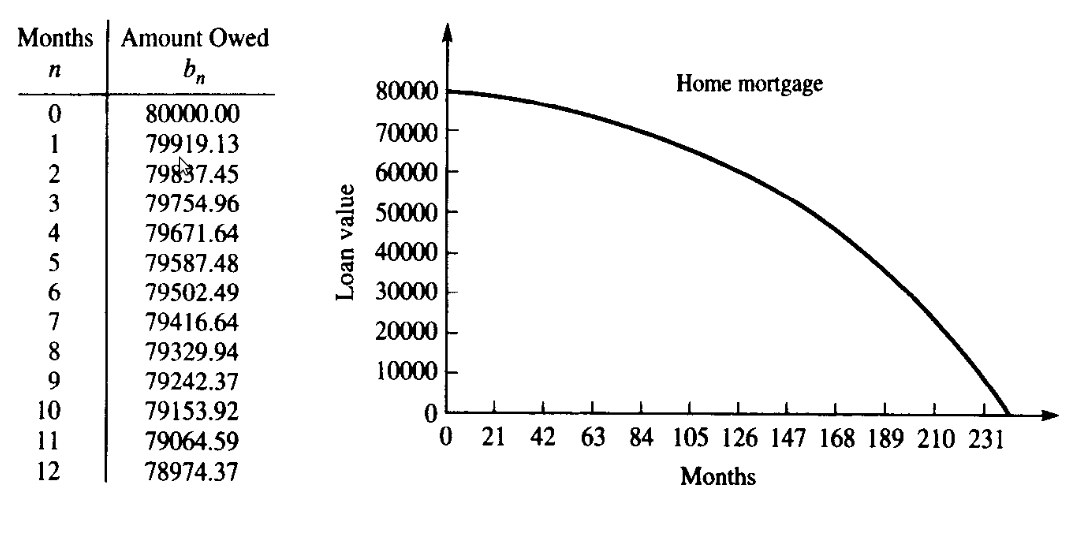
\includegraphics[width=.8\textwidth{}]{mort.png}
  \end{center}
\end{frame}

\begin{frame}{用差分方程来近似变化}

  \begin{itemize}
  \item 变化 = $\Delta a_n$ = 某个函数$f$
  \item 离散变化与连续变化
  \item 模型的细化: 生、死、资源
  \end{itemize}
\end{frame}

\begin{frame}{酵母培养 -- 找出模型}
  \begin{center}
    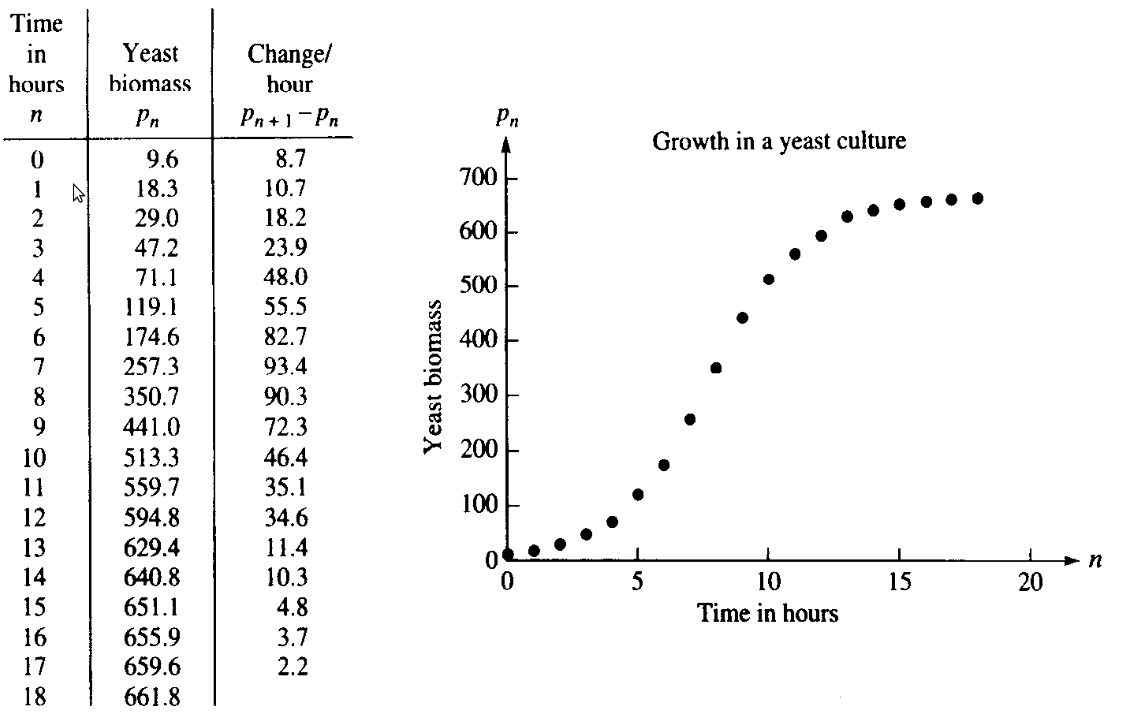
\includegraphics[width=.8\textwidth{}]{yeast.png}
  \end{center}

  \[
  \Delta p_n = p_{n+1} - p_n = k(665 - p_n)p_n
  \]
\end{frame}

\begin{frame}{酵母培养 -- 模型数值求解}
  \begin{center}
    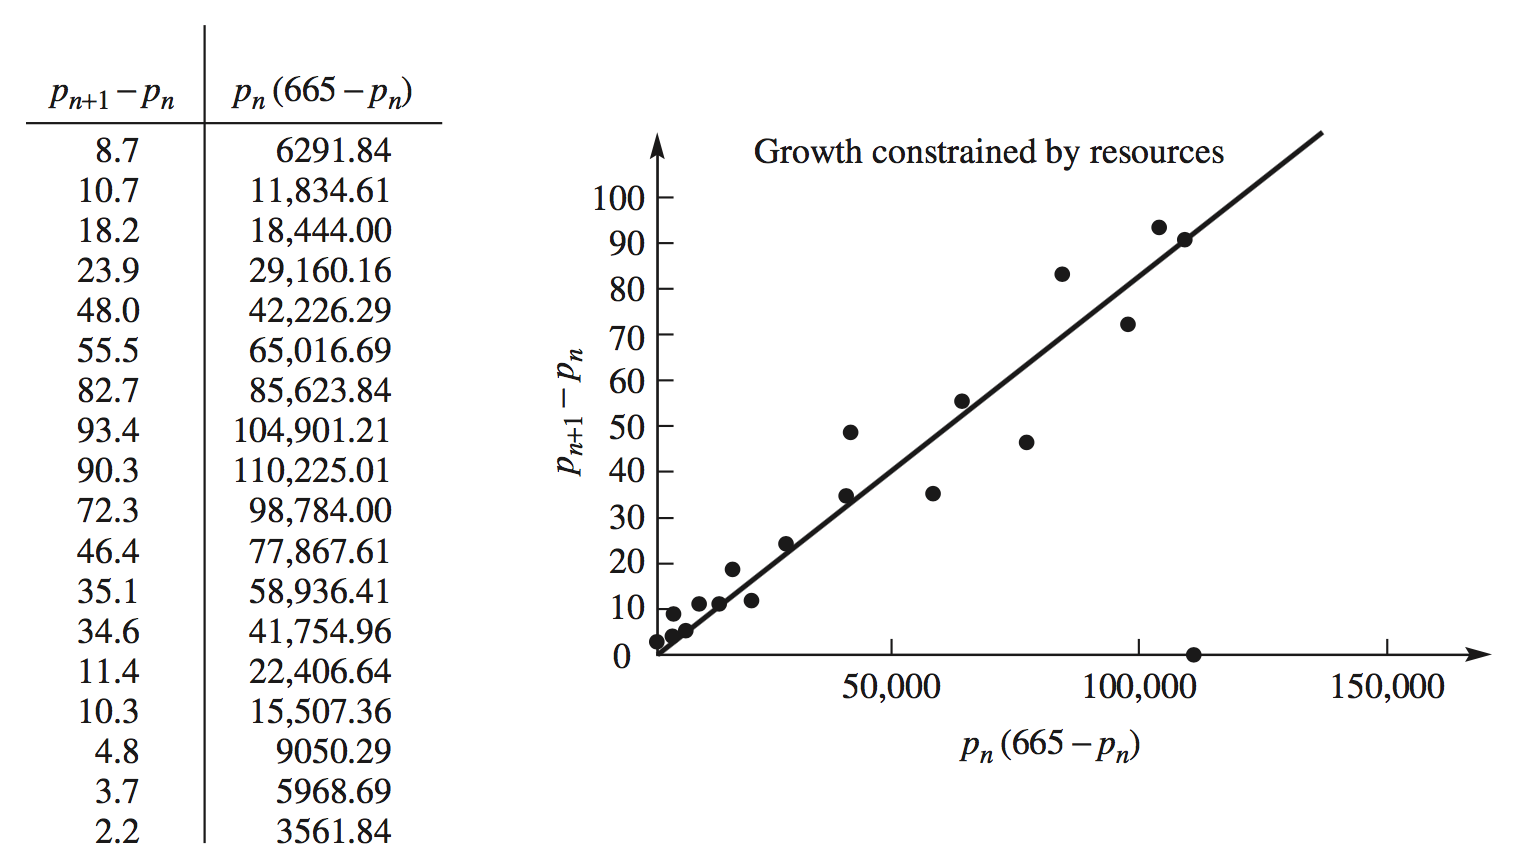
\includegraphics[width=.8\textwidth{}]{yeast-fit.png}
  \end{center}
  \[
  k \approx 0.00082
  \]
  \[
  p_{n+1} = p_n + 0.00082(665 - p_n)p_n
  \]  
\end{frame}

\begin{frame}{酵母培养 -- 模型验证}
  \begin{center}
    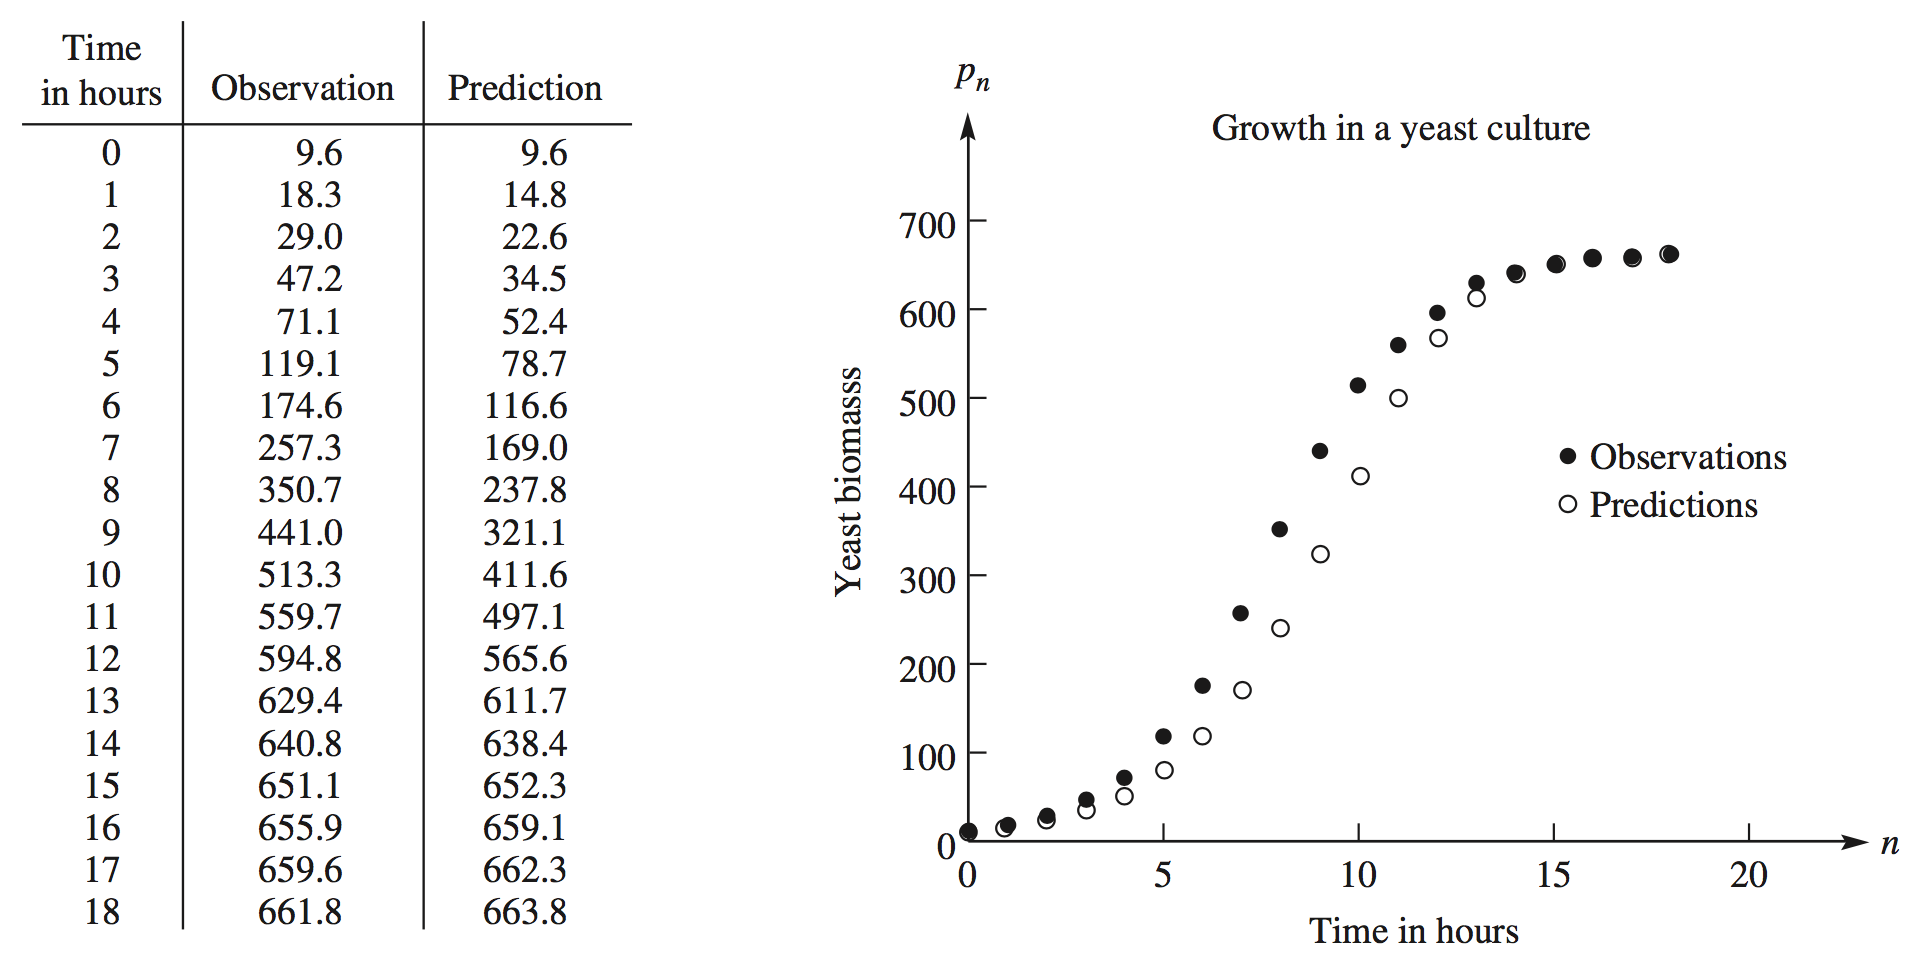
\includegraphics[width=.8\textwidth{}]{yeast-verify.png}
  \end{center}
  \[
  p_{n+1} = p_n + 0.00082(665 - p_n)p_n
  \]

思考: 看书上例2传染病传播模型, 考虑如何为该模型加入其它因素?
\end{frame}

\begin{frame}{地高辛在血流中的变化}
  \begin{center}
    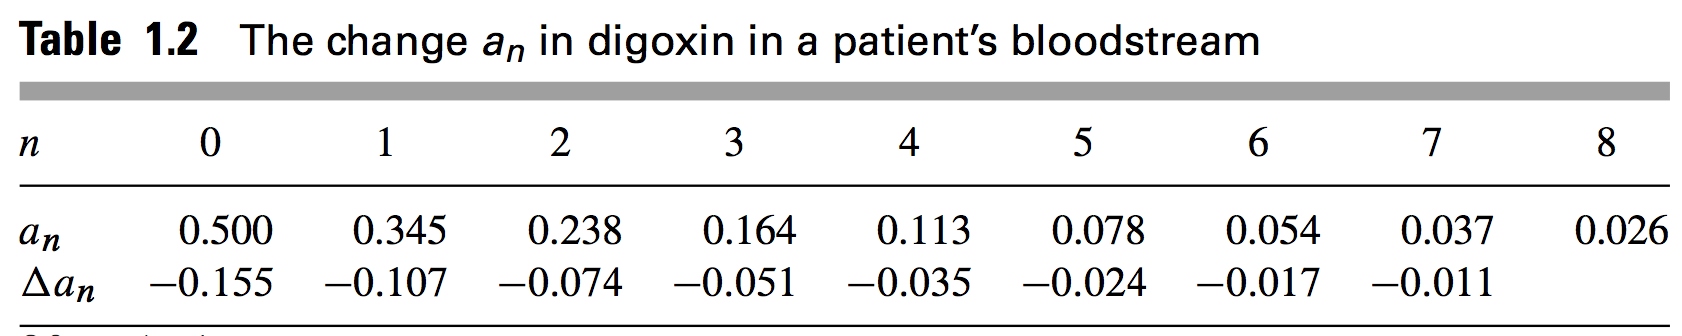
\includegraphics[width=.8\textwidth{}]{digoxin-table.png}\\
    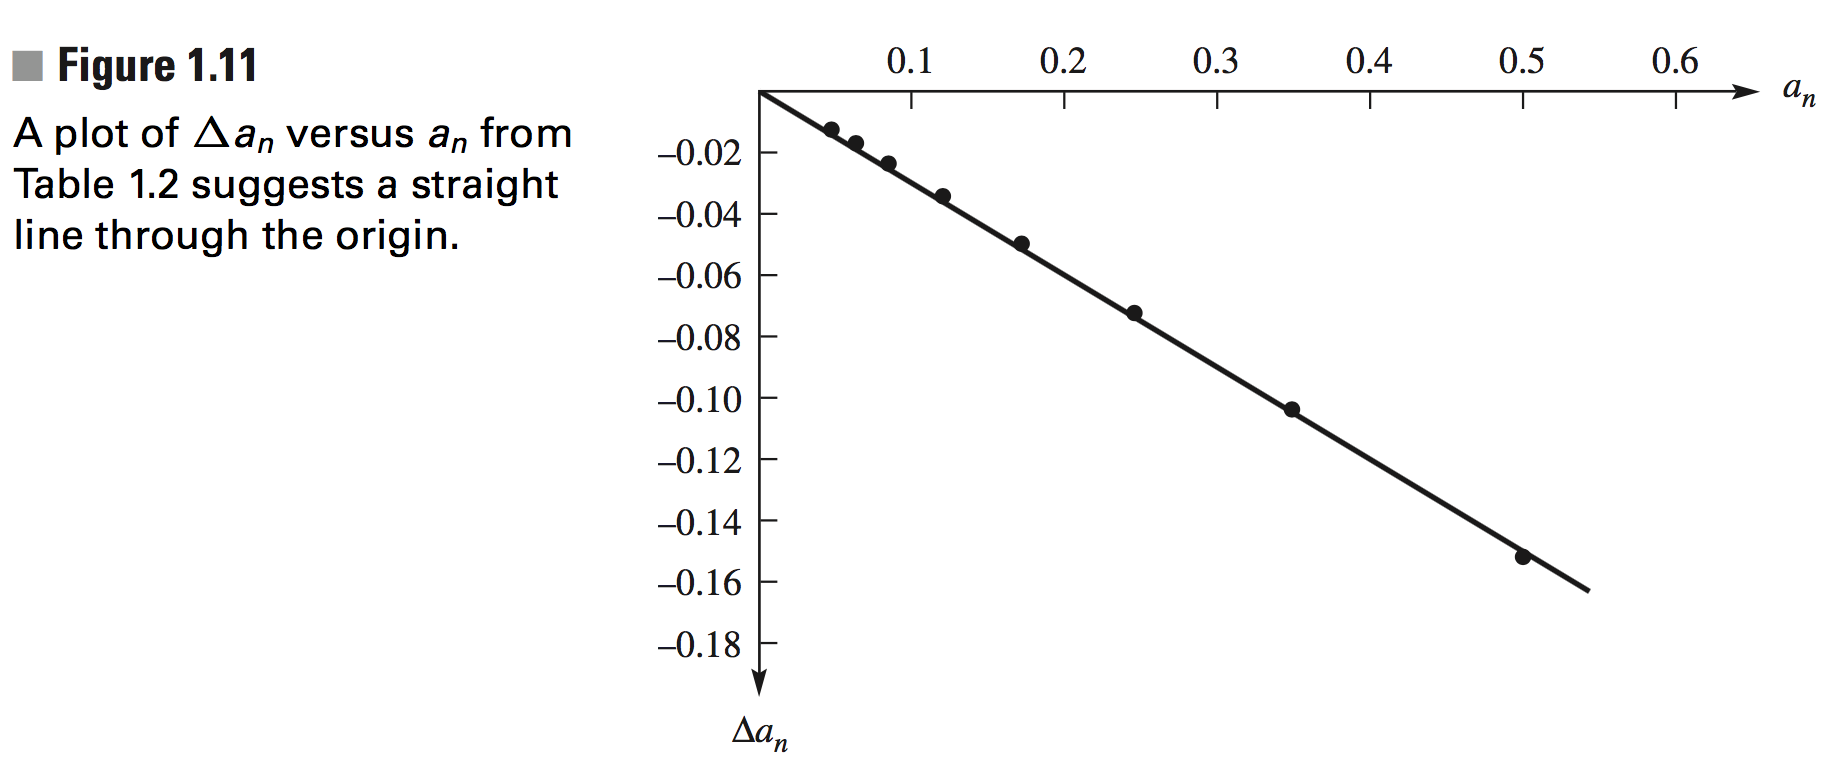
\includegraphics[width=.6\textwidth{}]{digoxin-fig.png}
  \end{center}
\[
\Delta a_n = -0.31a_n
\]\\[-25pt]
\[
a_{n+1} -  a_n = -0.31a_n
\]\\[-25pt]
\[
a_{n+1} = 0.69a_n
\]
\end{frame}

\begin{frame}{动态系统的解法 -- 猜测}
  存款问题: $a_{n+1} = 1.01a_n, a_0 = 1000$
  \begin{center}
    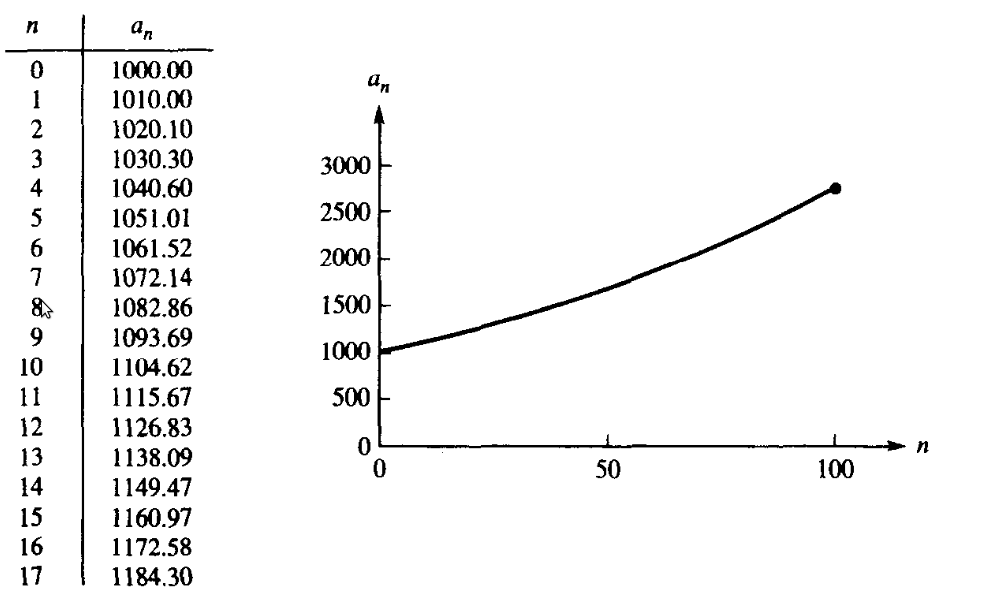
\includegraphics[width=.4\textwidth{}]{saving.png}
  \end{center}

$a_1 = 1010.0 = 1.01(1000)$\\
$a_2 = 1020.1 = 1.01(1010) = 1.01^2 (1000)$\\
$a_3 = 1030.3 = 1.01(1020.1) = 1.01^3 (1000)$\\
$a_4 = 1040.6 = 1.01(1030.3) = 1.01^4 (1000)$
\end{frame}

\begin{frame}{动态系统的解法 -- 猜测}
猜测: $a_k = 1.01^k(1000)$\\
验证、结论: ...

\begin{block}{推测法的一般步骤}
\begin{enumerate}
\item 观察模式
\item 猜测动力系统的形式
\item 用带入法来测试该猜测
\item 接受或拒绝该推测:取决于代入和代数运算后结果是否满足该动力系统。
\end{enumerate}
\end{block}

推论: 形式为$a_{n+1} = ra_n$的动态系统的解为$a_k = r^k a_0$.

\end{frame}

\begin{frame}{$a_{n+1}=ra_n$}

  $r = ?$
  \begin{center}
    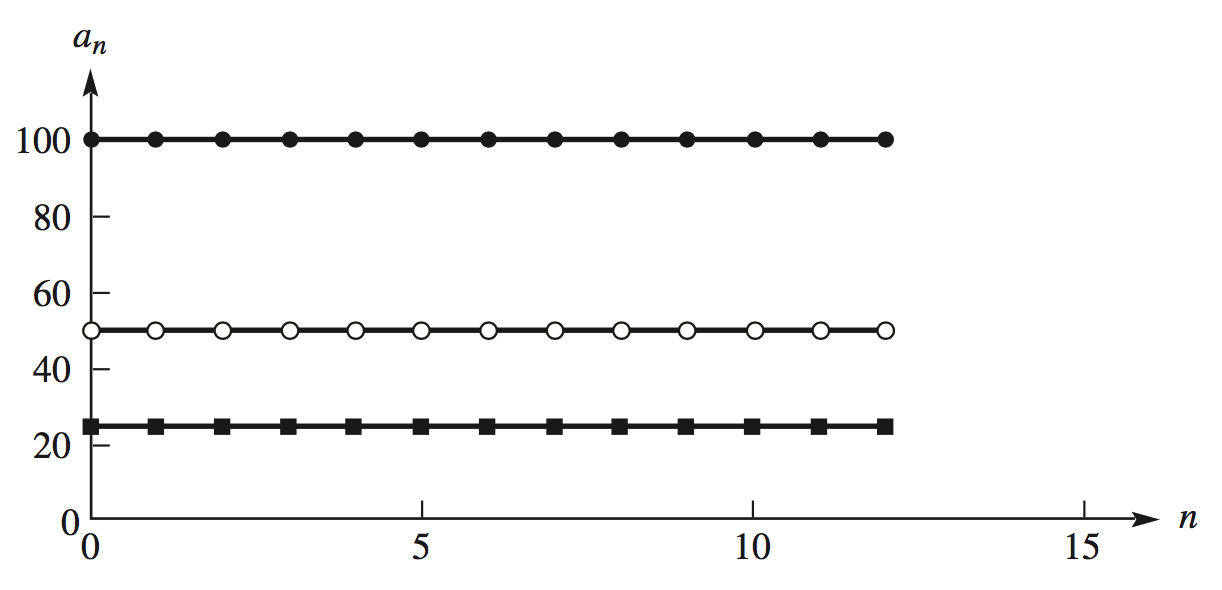
\includegraphics[width=.4\textwidth{}]{r0.png}
    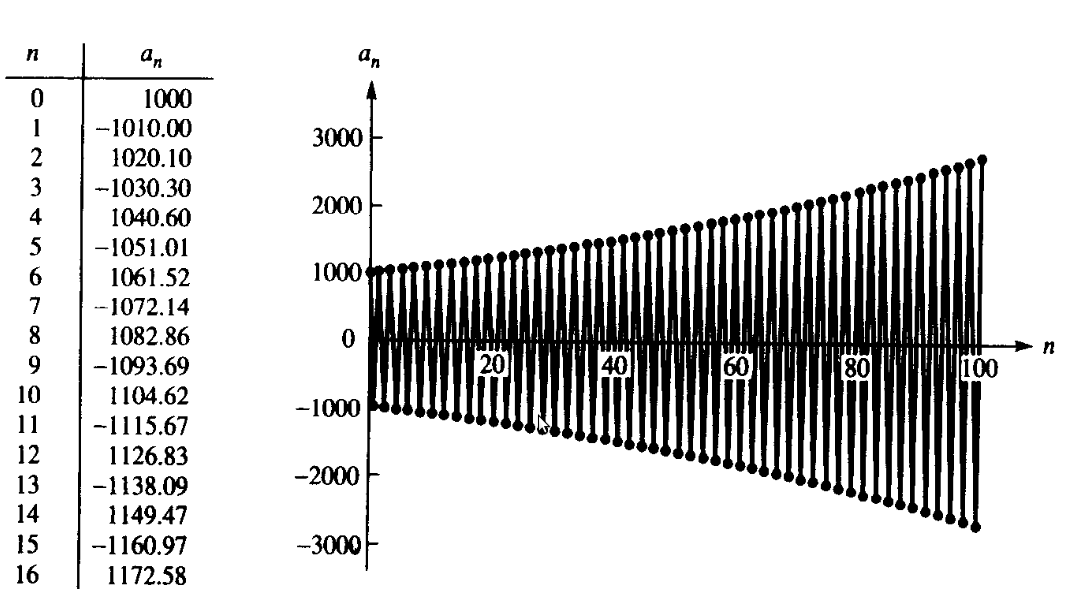
\includegraphics[width=.4\textwidth{}]{rn.png}
  \end{center}

  \begin{center}
    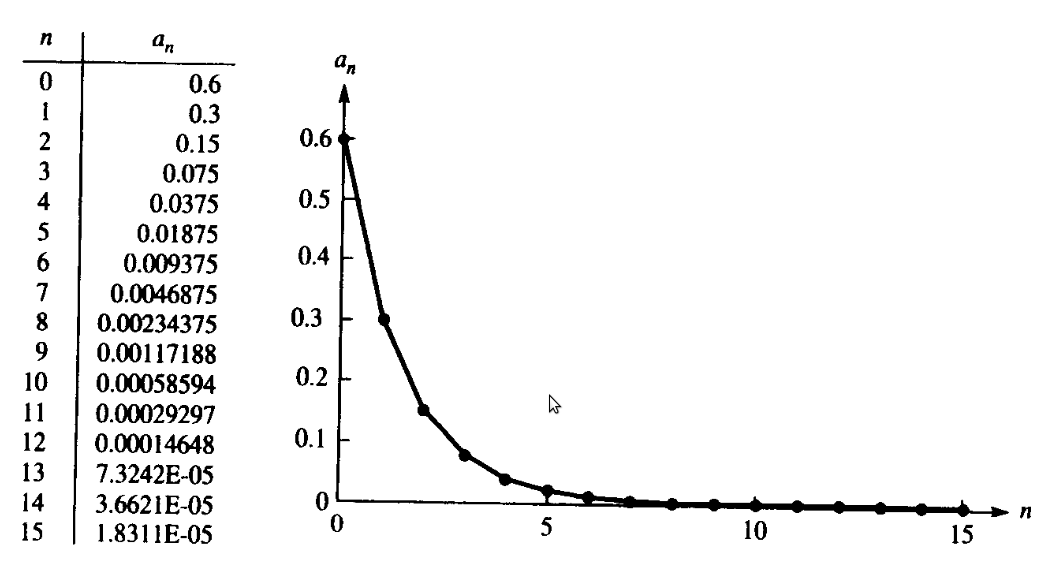
\includegraphics[width=.4\textwidth{}]{rf.png}
    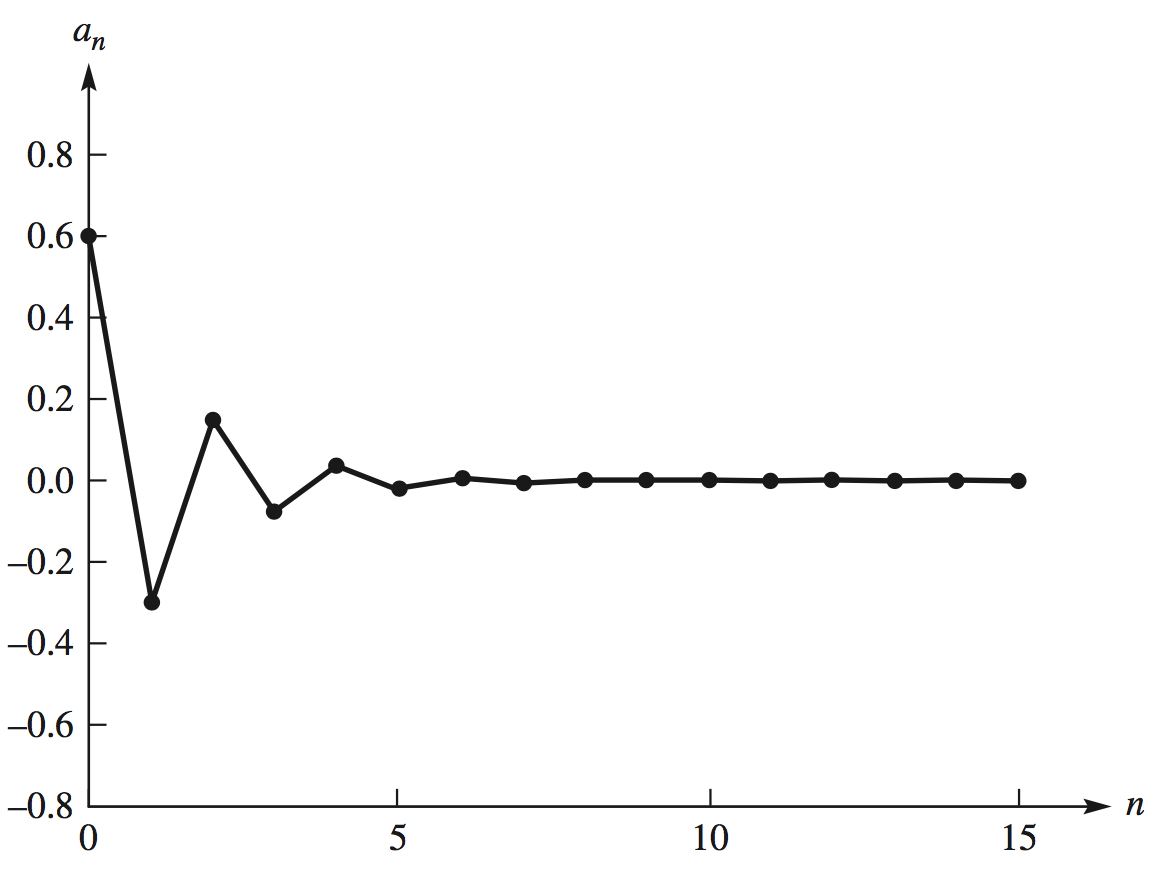
\includegraphics[width=.4\textwidth{}]{rnf.png}
  \end{center}
  
\end{frame}

\begin{frame}{$a_{n+1}=ra_n + b$}
  \begin{center}
    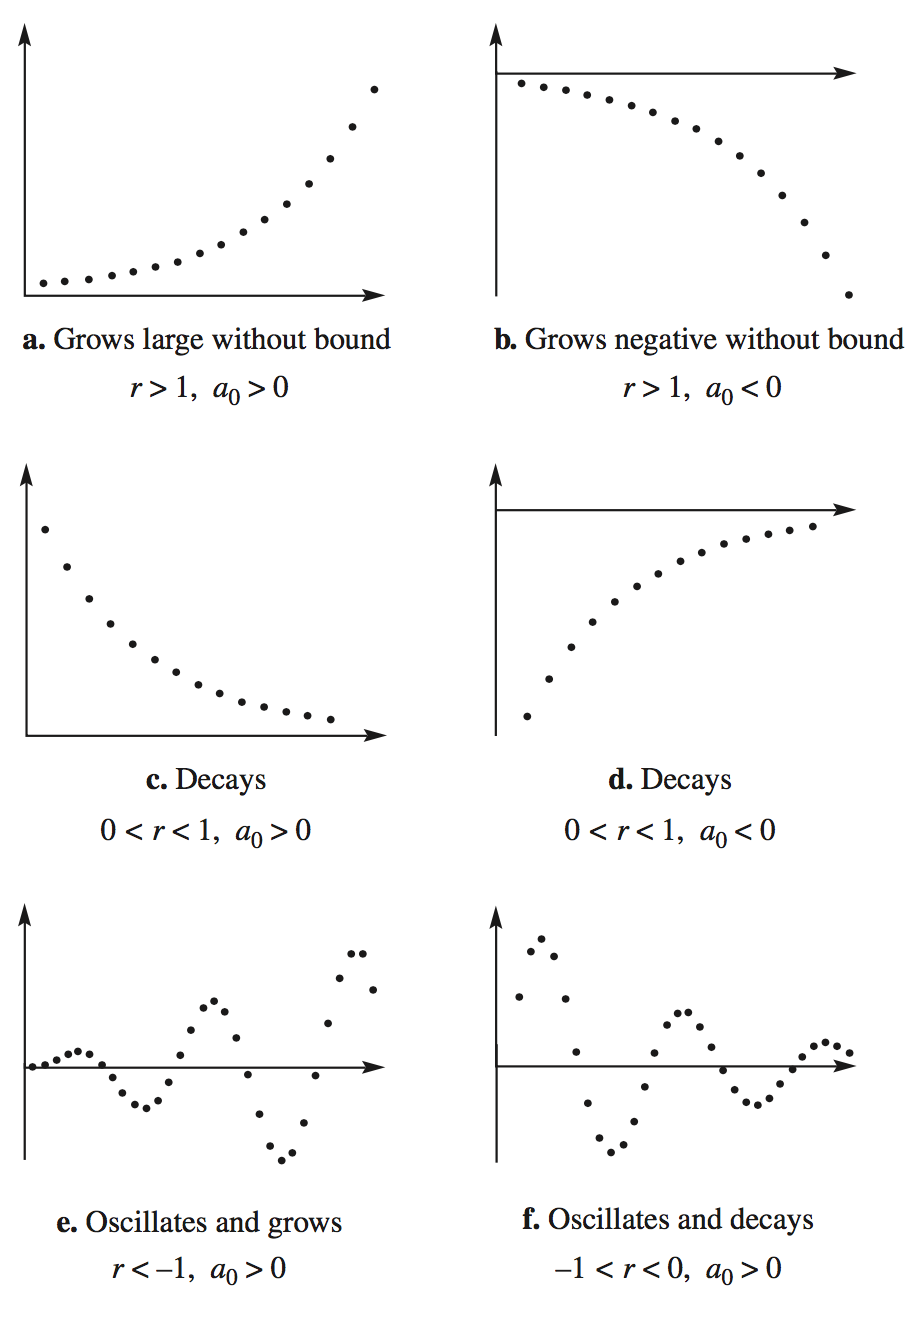
\includegraphics[width=.4\textwidth{}]{rb.png}
  \end{center}
\end{frame}

\begin{frame}{不动点(平衡点)}
  \begin{center}
    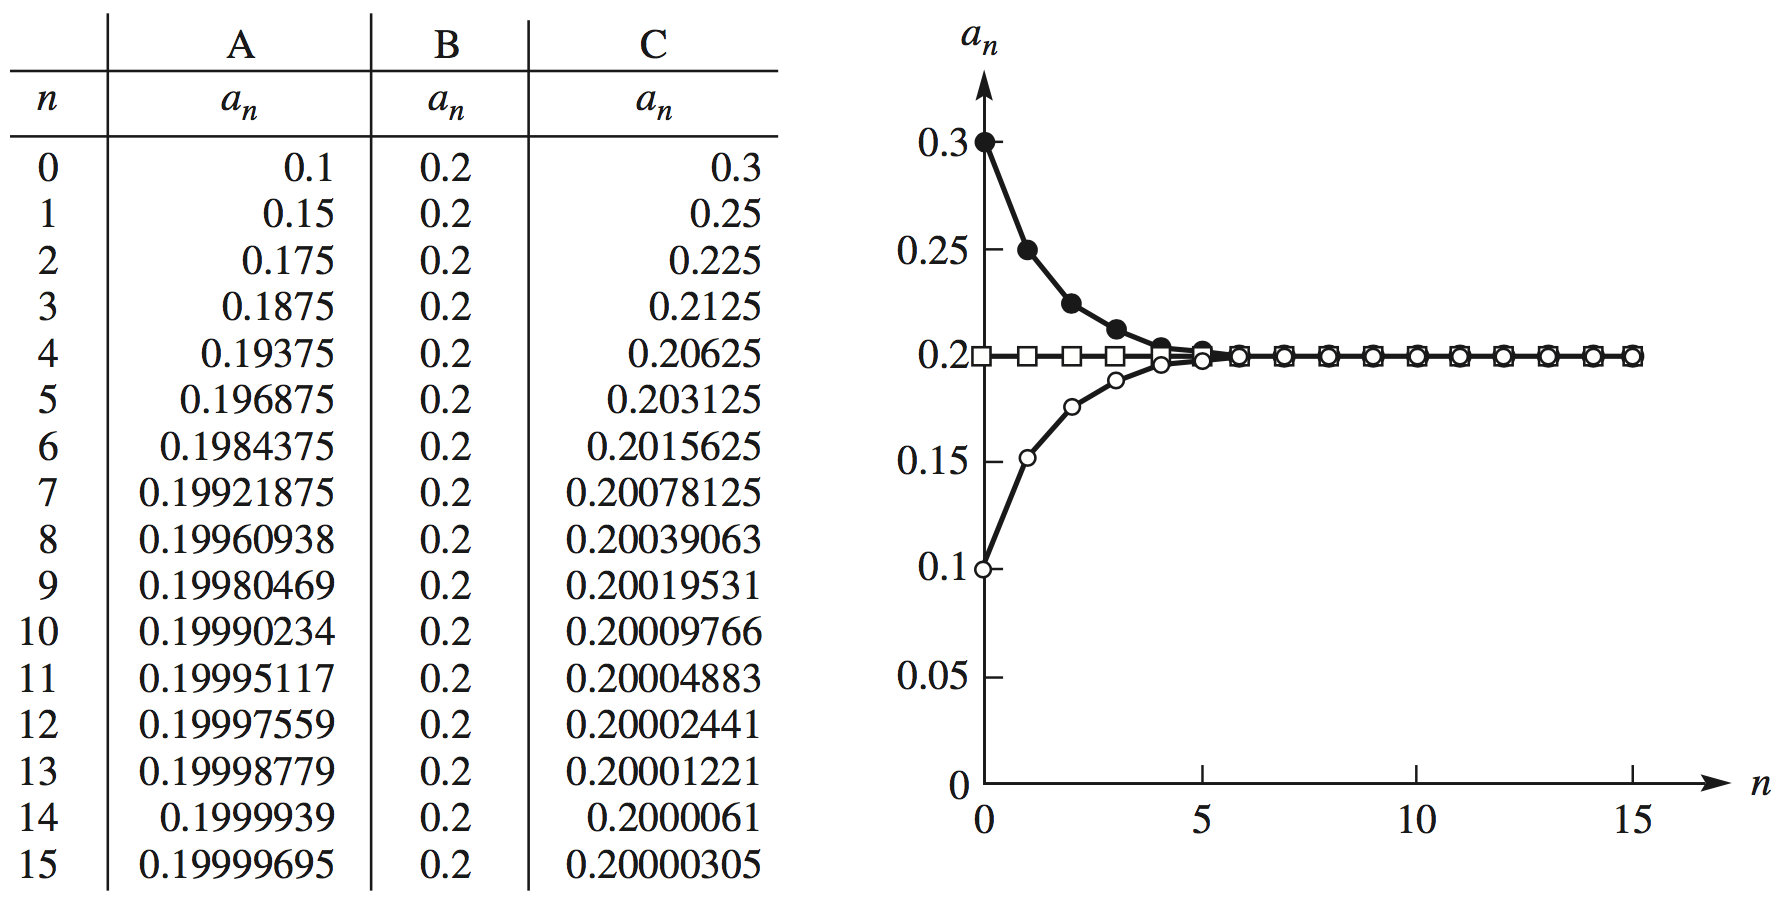
\includegraphics[width=.8\textwidth{}]{fixedpoint.png}\\
    Digoxin浓度变化
  \end{center}
  
\end{frame}

\begin{frame}{不动点}
\[
a_{n+1} = 1.01a_n -1000
\]
  \begin{center}
    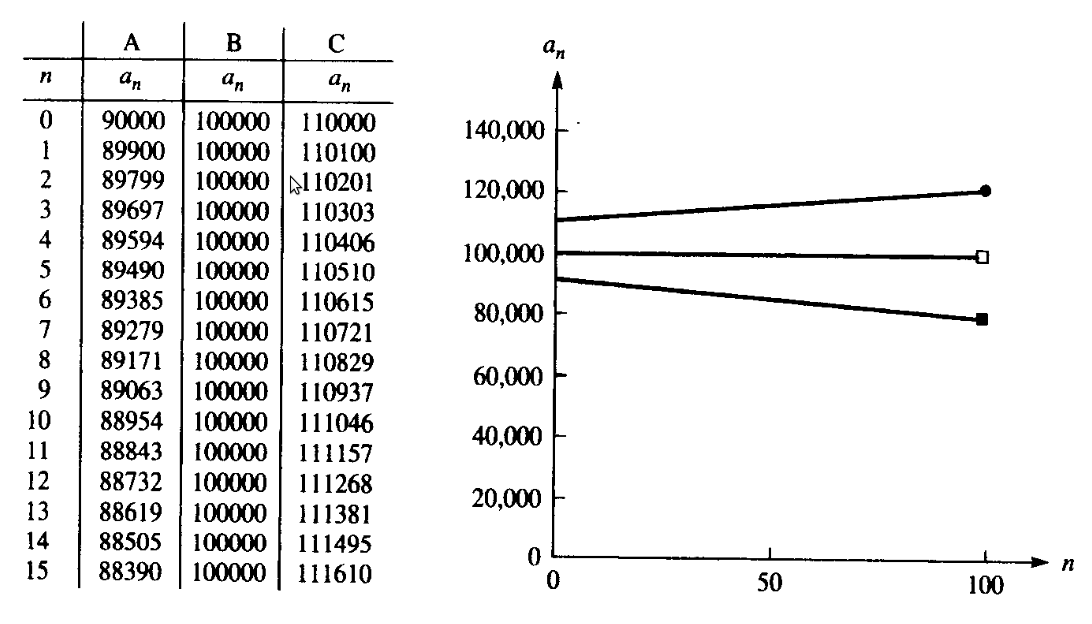
\includegraphics[width=.8\textwidth{}]{invest.png}\\
    投资
  \end{center}
  
\end{frame}

\begin{frame}{$r = 1$}
\[
a_{n+1} = a_n -300
\]
  \begin{center}
    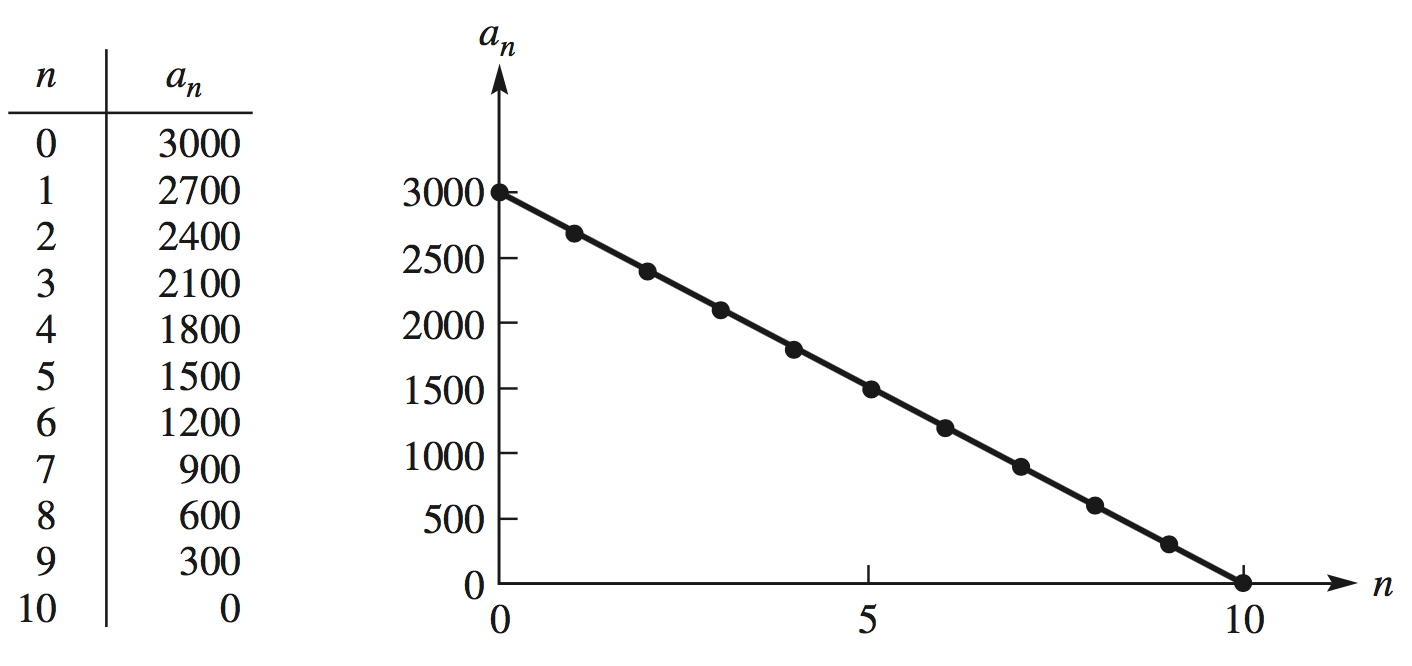
\includegraphics[width=.8\textwidth{}]{poor.png}
  \end{center}
  
\end{frame}

\begin{frame}{不动点}

$a_{n+1} = ra_n + b, r \neq 1$的不动点为:

\[
a = \frac{b}{1-r}
\]

上述动态系统的解为: $a_k=r^kc+\frac{b}{1-r}$.

思考: $r$的值不同时,长期来说系统如何变化?
  
\end{frame}

\begin{frame}{非线性系统}
  \begin{center}
    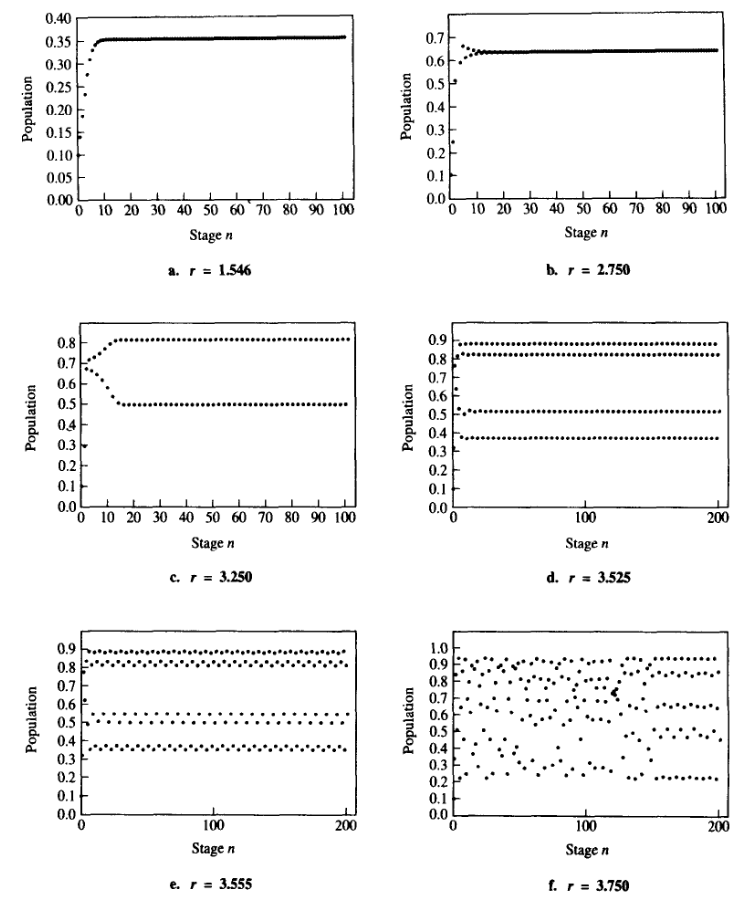
\includegraphics[width=.5\textwidth{}]{nonlinear.png}\\
  \end{center}
  
\end{frame}

\begin{frame}{差分方程组}
  \begin{itemize}
  \item 找出不动点
  \item 当初始值在不动点附近时,系统如何变化
  \end{itemize}

研究系统的长期变化,看系统对如下条件是否敏感:
\begin{itemize}
\item 初始条件
\item 对模型中的常量进行扰动
\end{itemize}

\end{frame}

\begin{frame}{汽车租赁公司}
  \begin{center}
    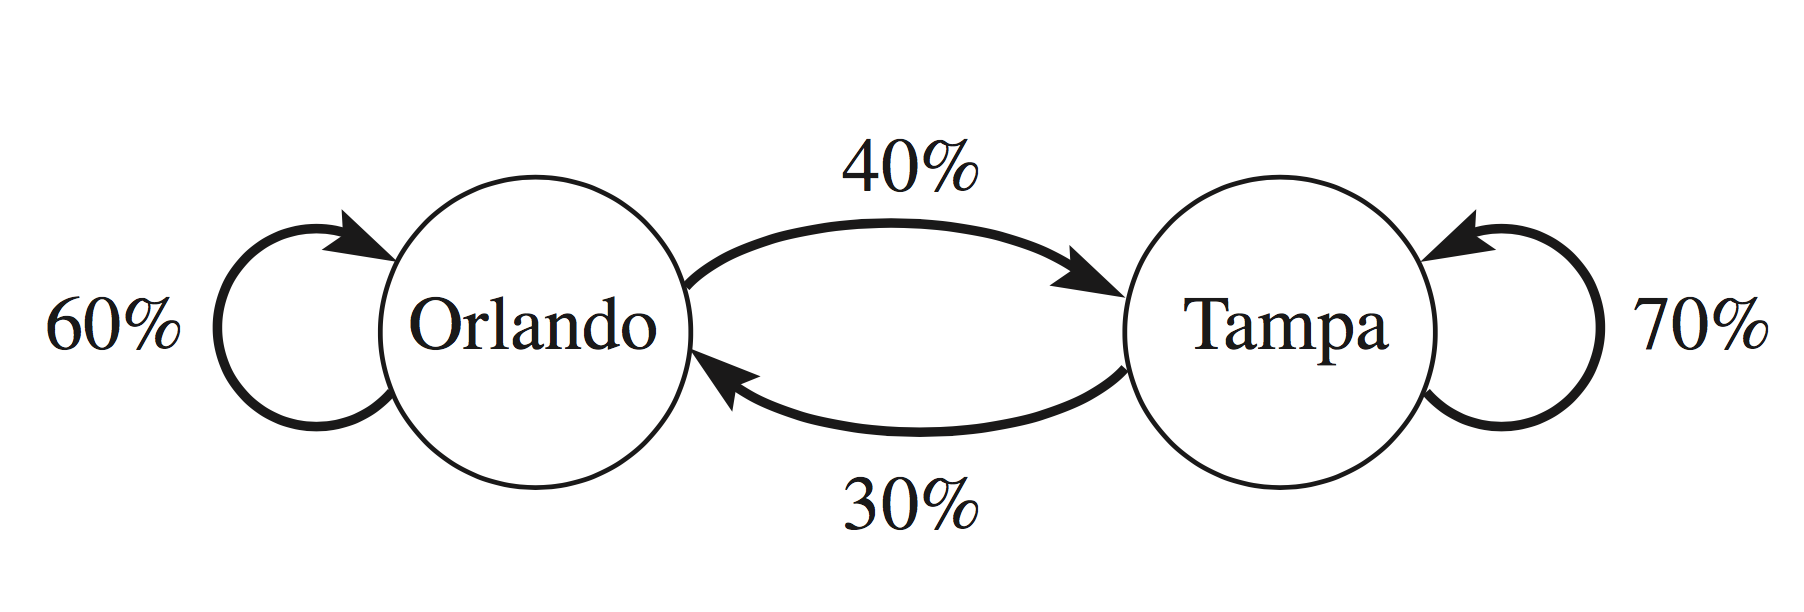
\includegraphics[width=.35\textwidth{}]{taxi.png}
  \end{center}
  \begin{definition}
    \begin{itemize}
    \item $O_n =$ 第$n$天营业结束时在奥兰多的车辆数
    \item $T_n =$ 第$n$天营业结束时在坦帕的车辆数
    \end{itemize}
  \end{definition}
  \[
  O_{n+1}=0.6O_n + 0.3T_n
  \]
  \[
  T_{n+1}=0.4O_n + 0.7T_n
  \]
\end{frame}

\begin{frame}{计算平衡点}
  如果存在平衡点$O$, $T$:
  \[
  O=O_{n+1}=O_n
  \]
  \[
  T=T_{n+1}=T_n
  \]
  推导出:
  \[
  O=0.6O + 0.3T
  \]
  \[
  T=0.4O + 0.7T
  \]
\end{frame}

\begin{frame}{方程求解}
  $O=\frac{3}{4}T$满足上述方程组. 如果公司有7000辆车,则$(O, T) = (3000, 4000)$处开始,保持不变。

  分析下述四种初始条件:

  \begin{center}
    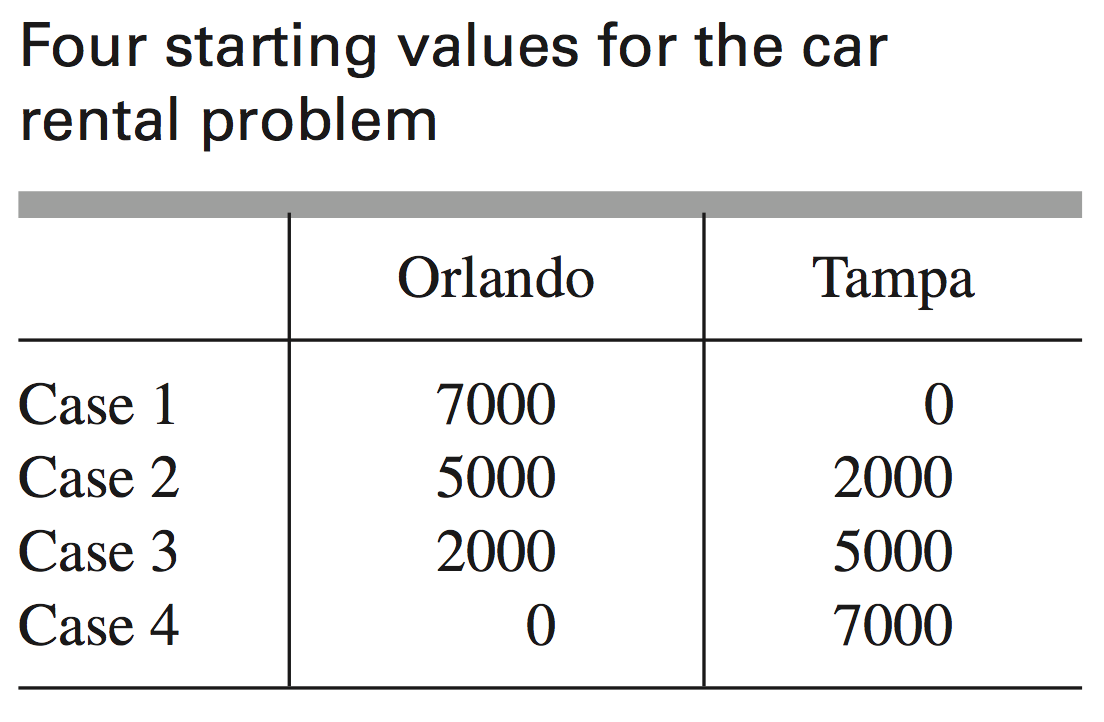
\includegraphics[width=.4\textwidth{}]{taxi-cases.png}
  \end{center}

\end{frame}

\begin{frame}{分析}
  \begin{center}
    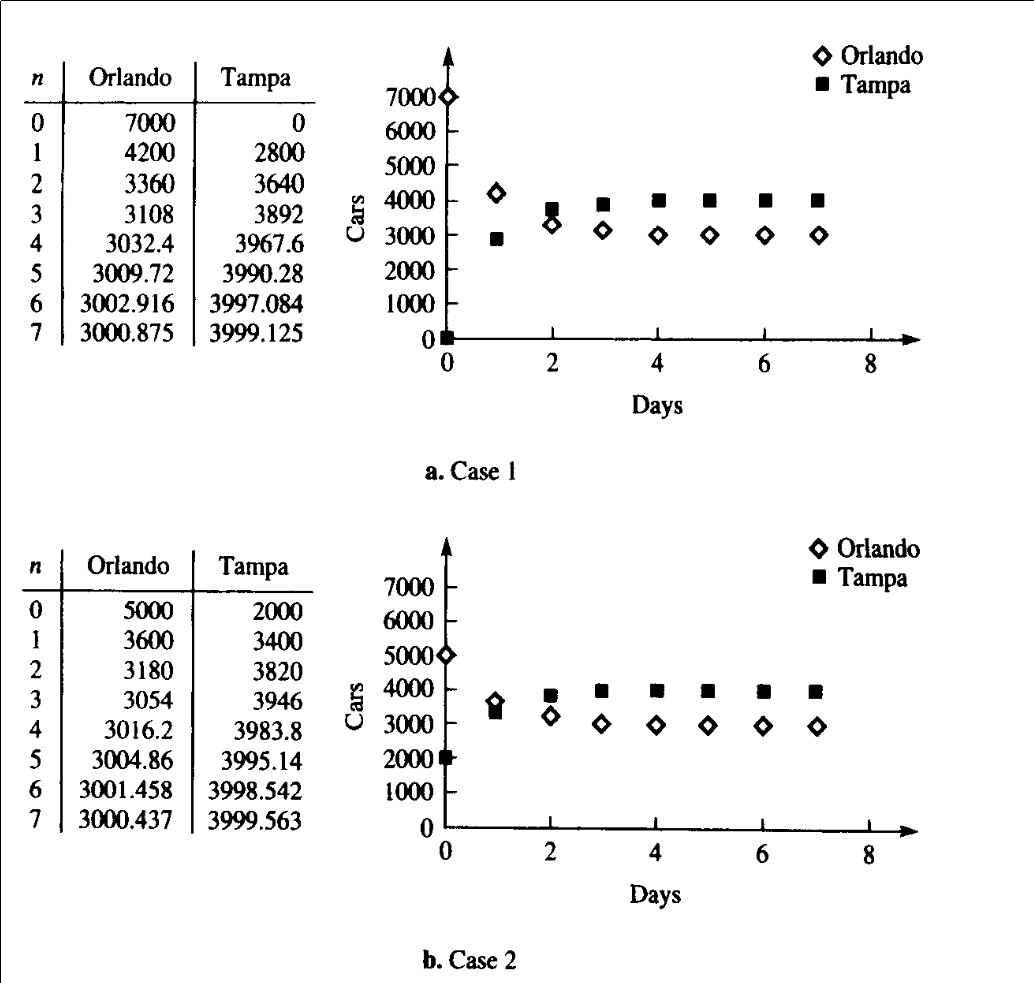
\includegraphics[width=.6\textwidth{}]{taxi-case12.png}
  \end{center}
\end{frame}

\begin{frame}{分析}
  \begin{center}
    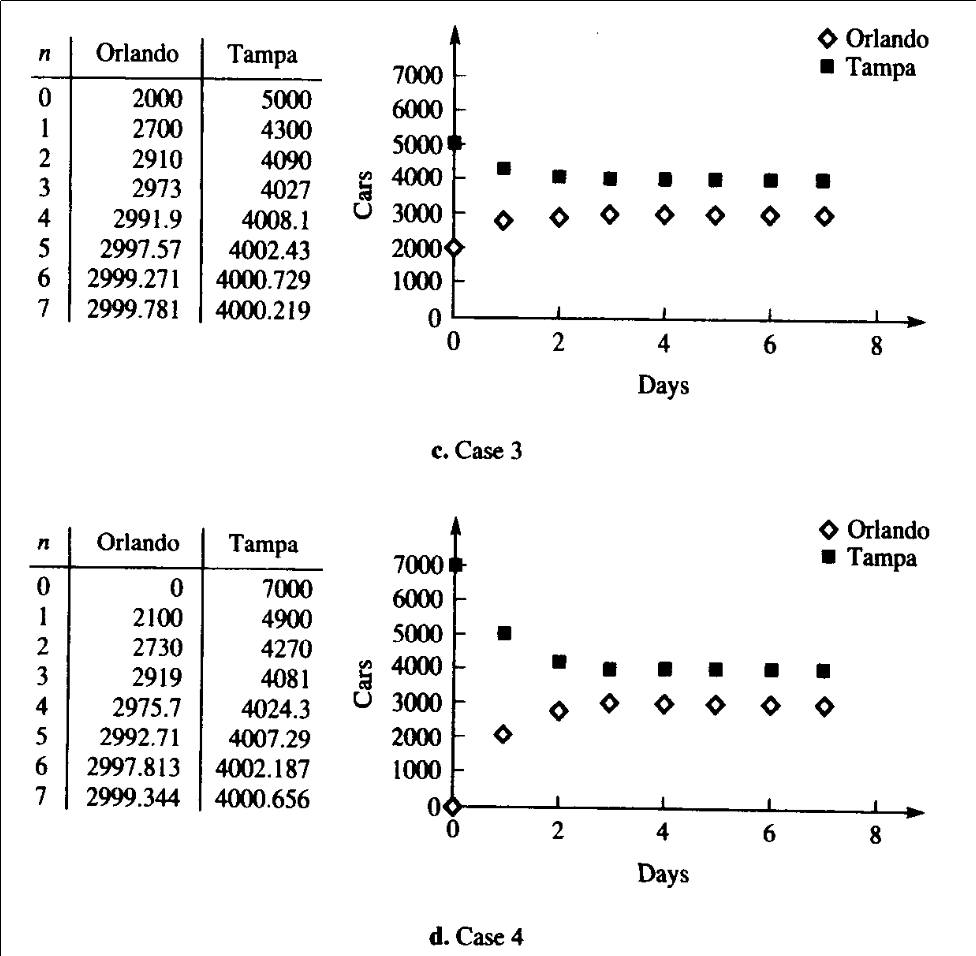
\includegraphics[width=.6\textwidth{}]{taxi-case34.png}
  \end{center}
\end{frame}

\begin{frame}{结论}
  四种情形中每一种情形在一周内都是和平衡点$(3000,4000)$很接近的,甚至在其中一个城市没有车的情况也是如此。结果显示,平衡点是稳定的而且对初始值不敏感的。

  思考:该系统是否对$O_{n+1}$和$T_{n+1}$的系数敏感?

\end{frame}

\begin{frame}{特拉法尔加战斗}

  法西联军33艘战舰,英军27艘战舰,在一次遭遇战中每方的战舰损失都是对方战舰的$10\%$。

  {\bf{}动力系统模型} 令$n$表示战斗过程中遭遇战的阶段并定义:

  \begin{definition}
    \begin{itemize}
    \item $B_n = $第$n$阶段英军的战舰数
    \item $F_n = $第$n$阶段法西联军的战舰数
    \end{itemize}
  \end{definition}

\end{frame}

\begin{frame}{死拼打法}
  战斗结束:英军全面战败,剩3艘战舰其中一艘严重损坏,法军大约还有18艘战舰。
  \begin{center}
    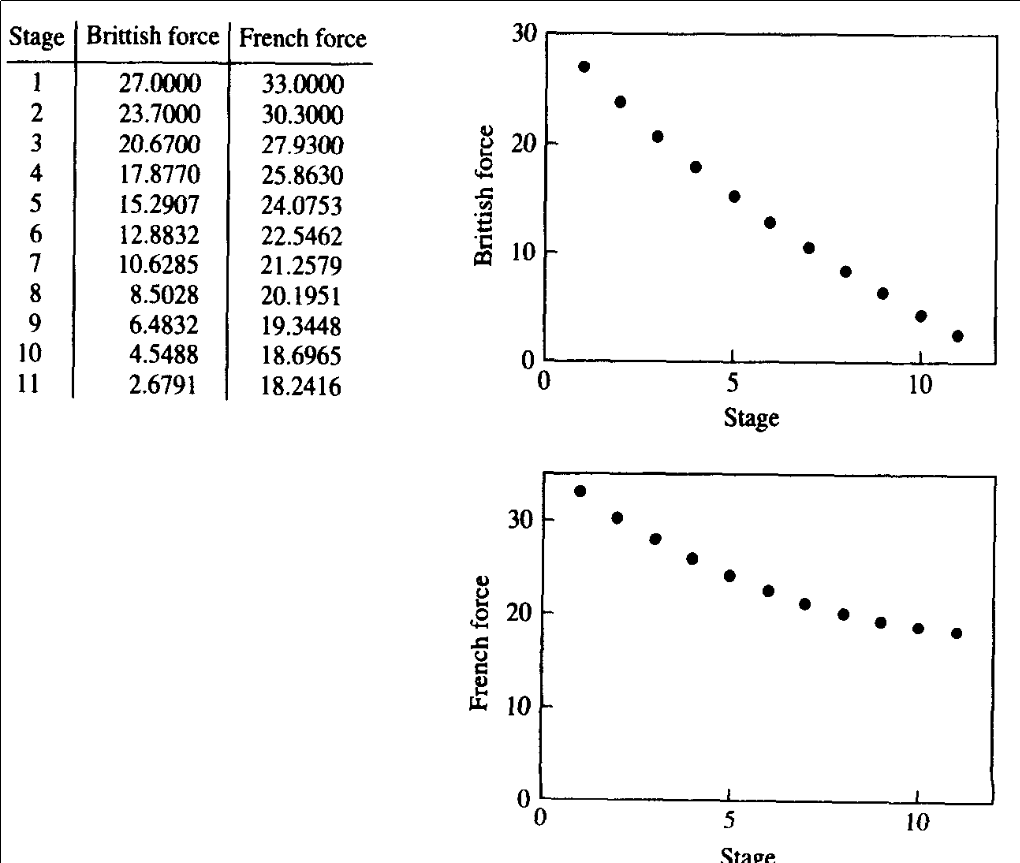
\includegraphics[width=.6\textwidth{}]{fight-death.png}
  \end{center}
\end{frame}

\begin{frame}{各个击破}
  \begin{center}
    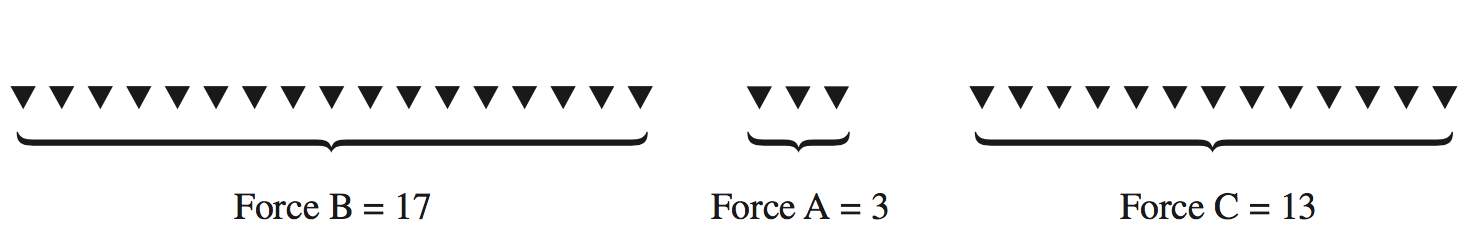
\includegraphics[width=.6\textwidth{}]{fight-france.png}
  \end{center}
  
  策略:英军13艘攻击$A$;然后,全力攻击$B$,最后攻击$C$。
  
\end{frame}

\begin{frame}{战斗A}
  \begin{center}
    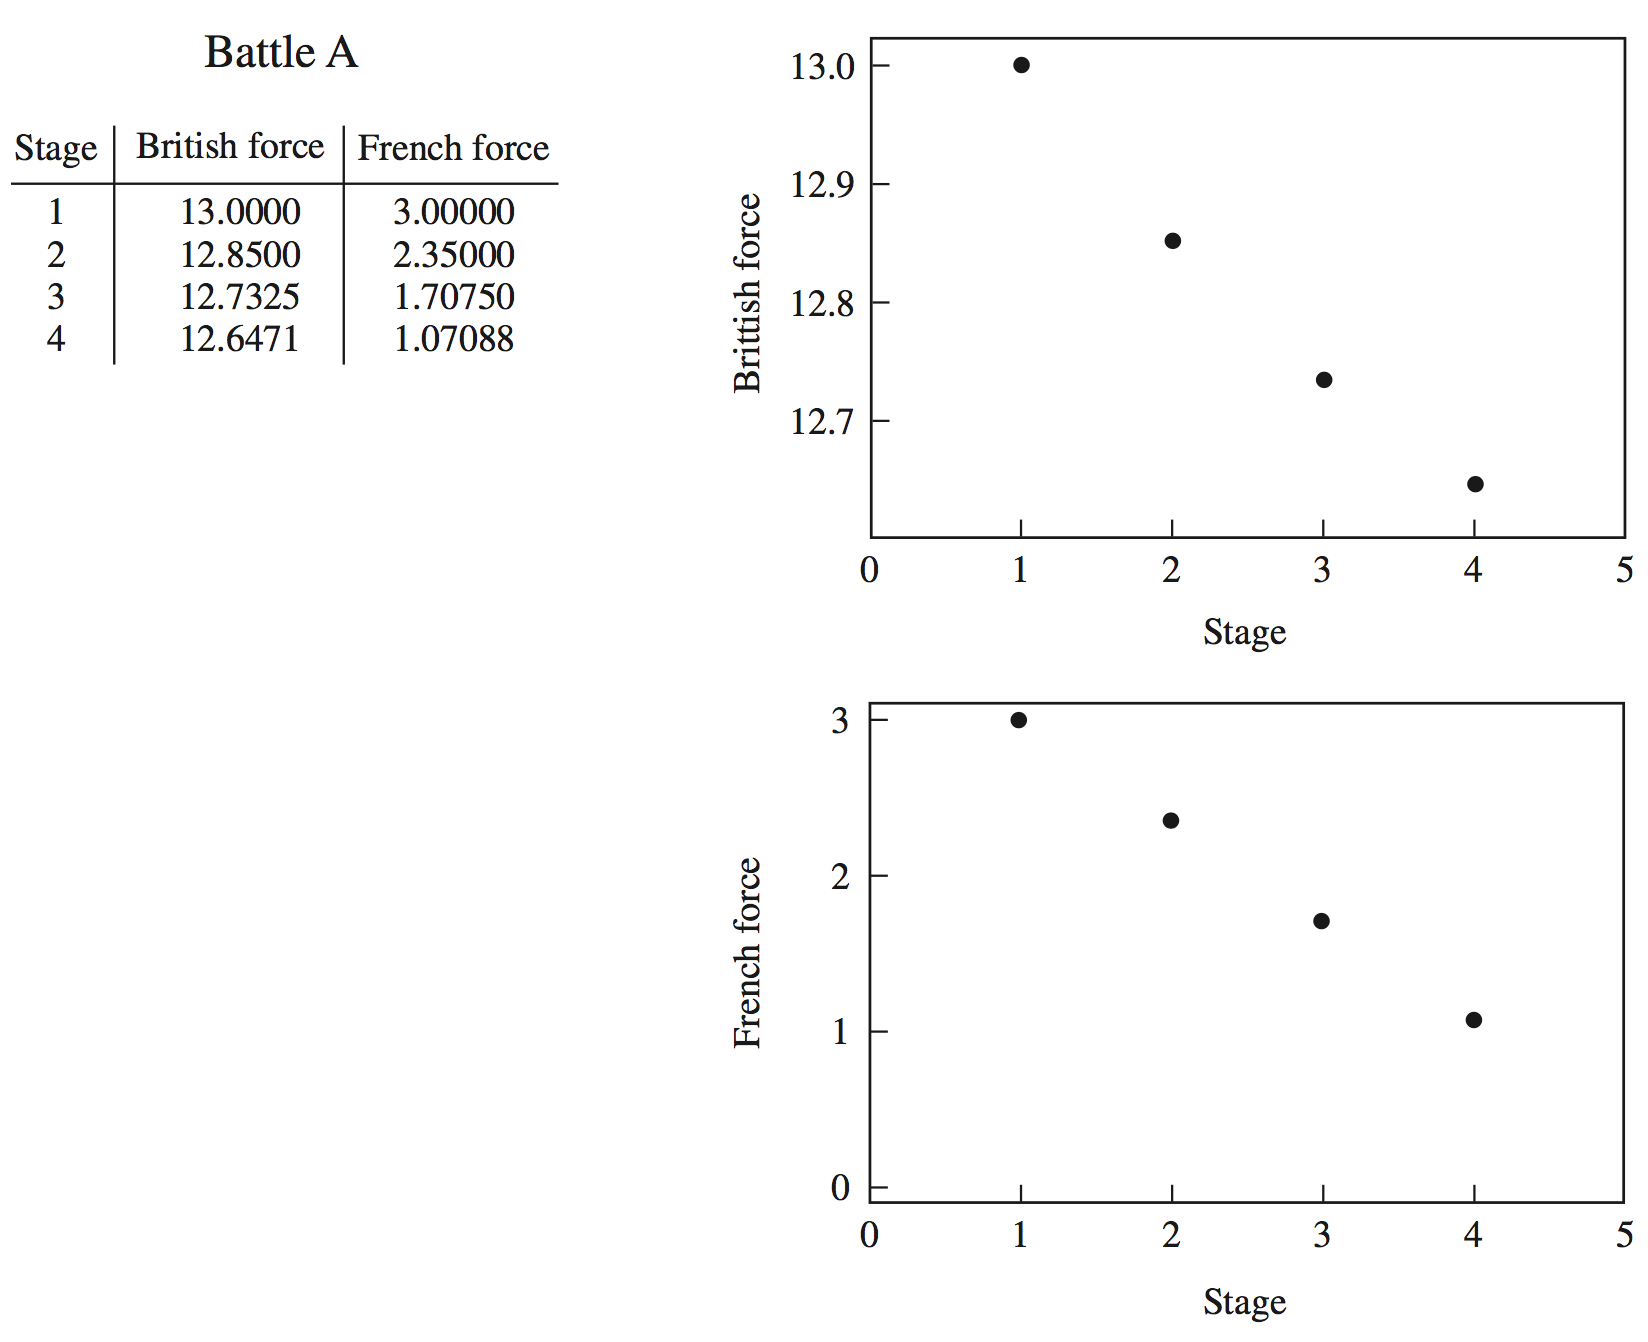
\includegraphics[height=.9\textheight{}]{fight-A.png}
  \end{center}  
\end{frame}

\begin{frame}{战斗B}
  \begin{center}
    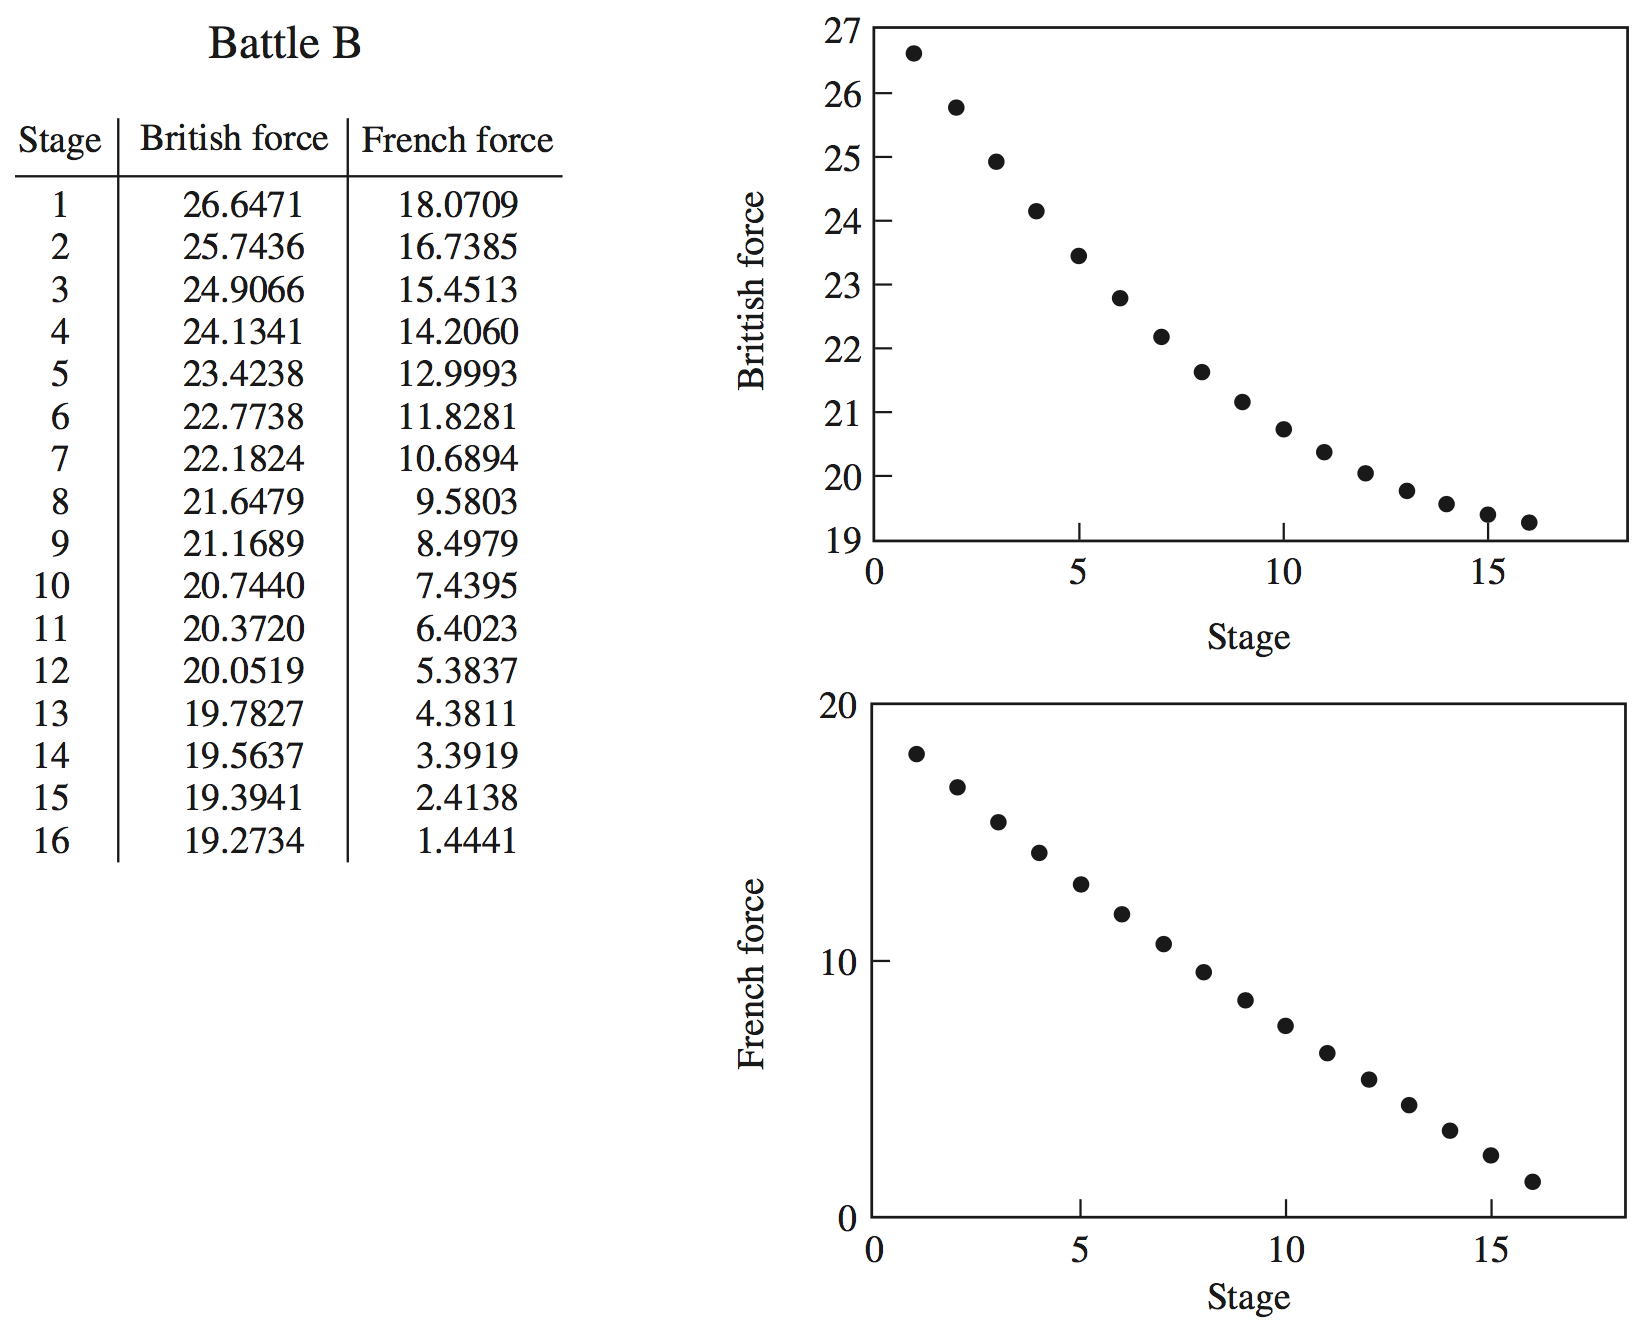
\includegraphics[height=.9\textheight{}]{fight-B.png}
  \end{center}  
\end{frame}

\begin{frame}{战斗C}
  \begin{center}
    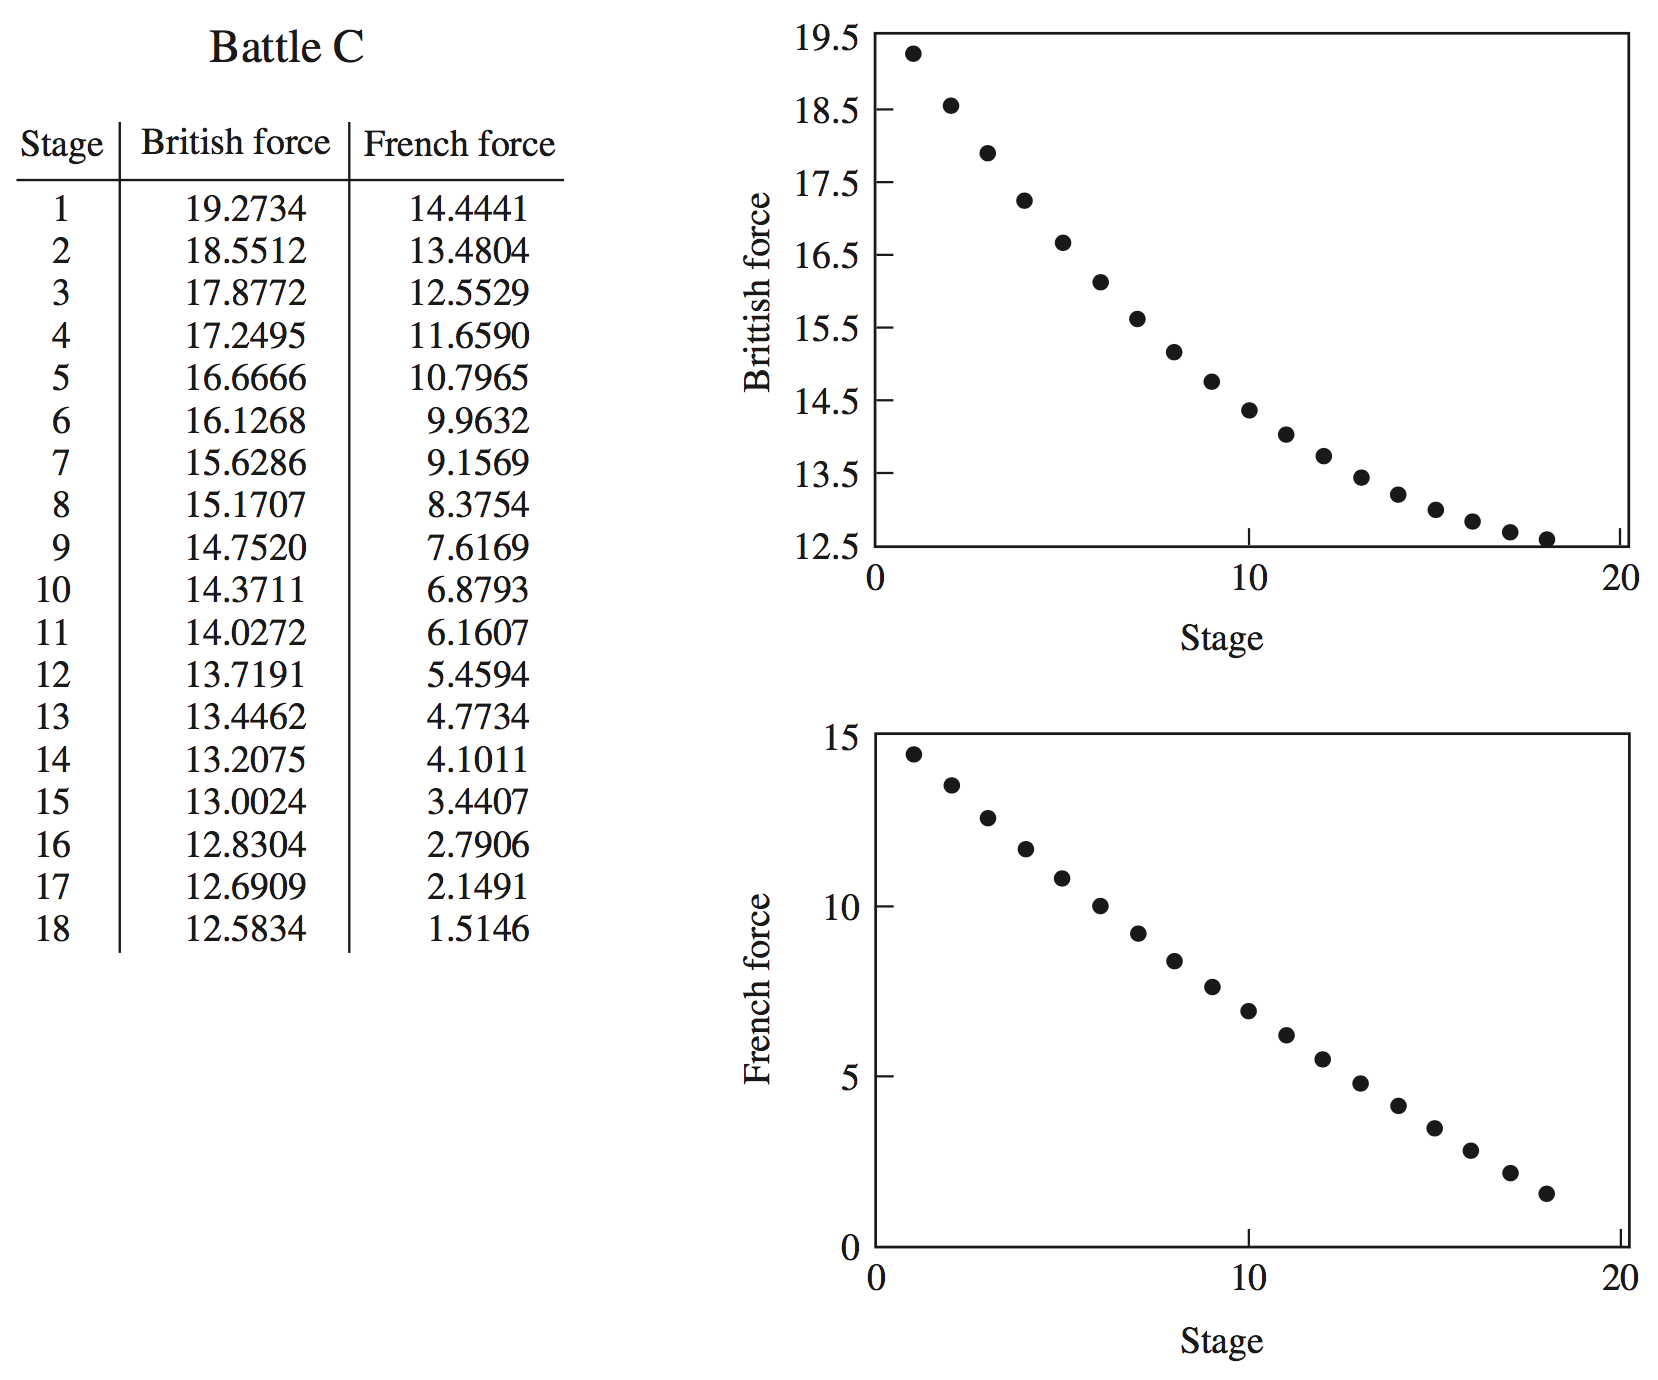
\includegraphics[height=.9\textheight{}]{fight-C.png}
  \end{center}  
\end{frame}

\begin{frame}{战果}
  英军大获全胜。现实世界:法西联军没有参加战斗C,而是把剩下的约13艘战舰撤回法国。

\end{frame}

\begin{frame}{斑点猫头鹰和隼}
  \begin{itemize}
  \item<1-> $O_n$, $H_n$分别表示第$n$天猫头鹰和隼的数量
  \item<2-> $\Delta O_n=k_1O_n$, $\Delta H_n=k_2H_n$ (不考虑竞争)
  \item<3-> $\Delta O_n=k_1O_n - k_3O_nH_n$, $\Delta H_n=k_2H_n-k_4O_nH_n$ (考虑竞争)
  \item<4-> $O_{n+1}=(1+k_1)O_n - k_3O_nH_n$
  \item<4-> $H_{n+1}=(1+k_2)H_n-k_4O_nH_n$
  \end{itemize}
  
\end{frame}

\begin{frame}{求解平衡点}
  \begin{definition}
    \begin{itemize}
    \item $O_{n+1}=1.2O_n - 0.001O_nH_n$
    \item $H_{n+1}=1.3H_n - 0.002O_nH_n$
    \end{itemize}
  \end{definition}

  如果$(O,H)$为平衡点则$O_{n+1}=O_n=O$, $H_{n+1}=H_n=H$:

  \begin{itemize}
  \item $O=1.2O - 0.001OH \Rightarrow O = 0 or H = 200$ 
  \item $H=1.3H - 0.002OH \Rightarrow H = 0 or O = 150$
  \end{itemize}

\end{frame}

\begin{frame}{平衡点分析}
  两个平衡点: $(0, 0)$, $(150, 200)$. 为什么?

  \begin{center}
    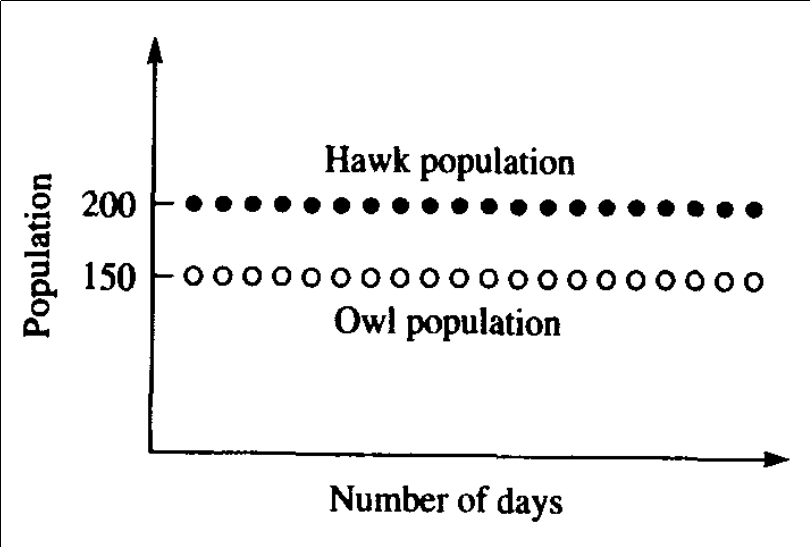
\includegraphics[width=.4\textwidth{}]{owl.png}
    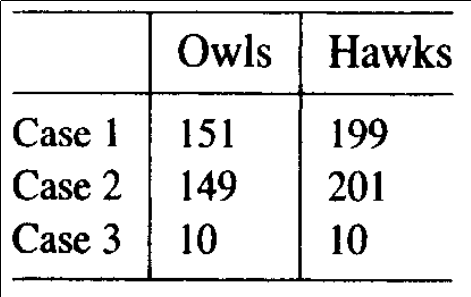
\includegraphics[height=.2\textwidth{}]{owl-start.png}
  \end{center}  

\end{frame}

\begin{frame}{情况1}
  \begin{center}
    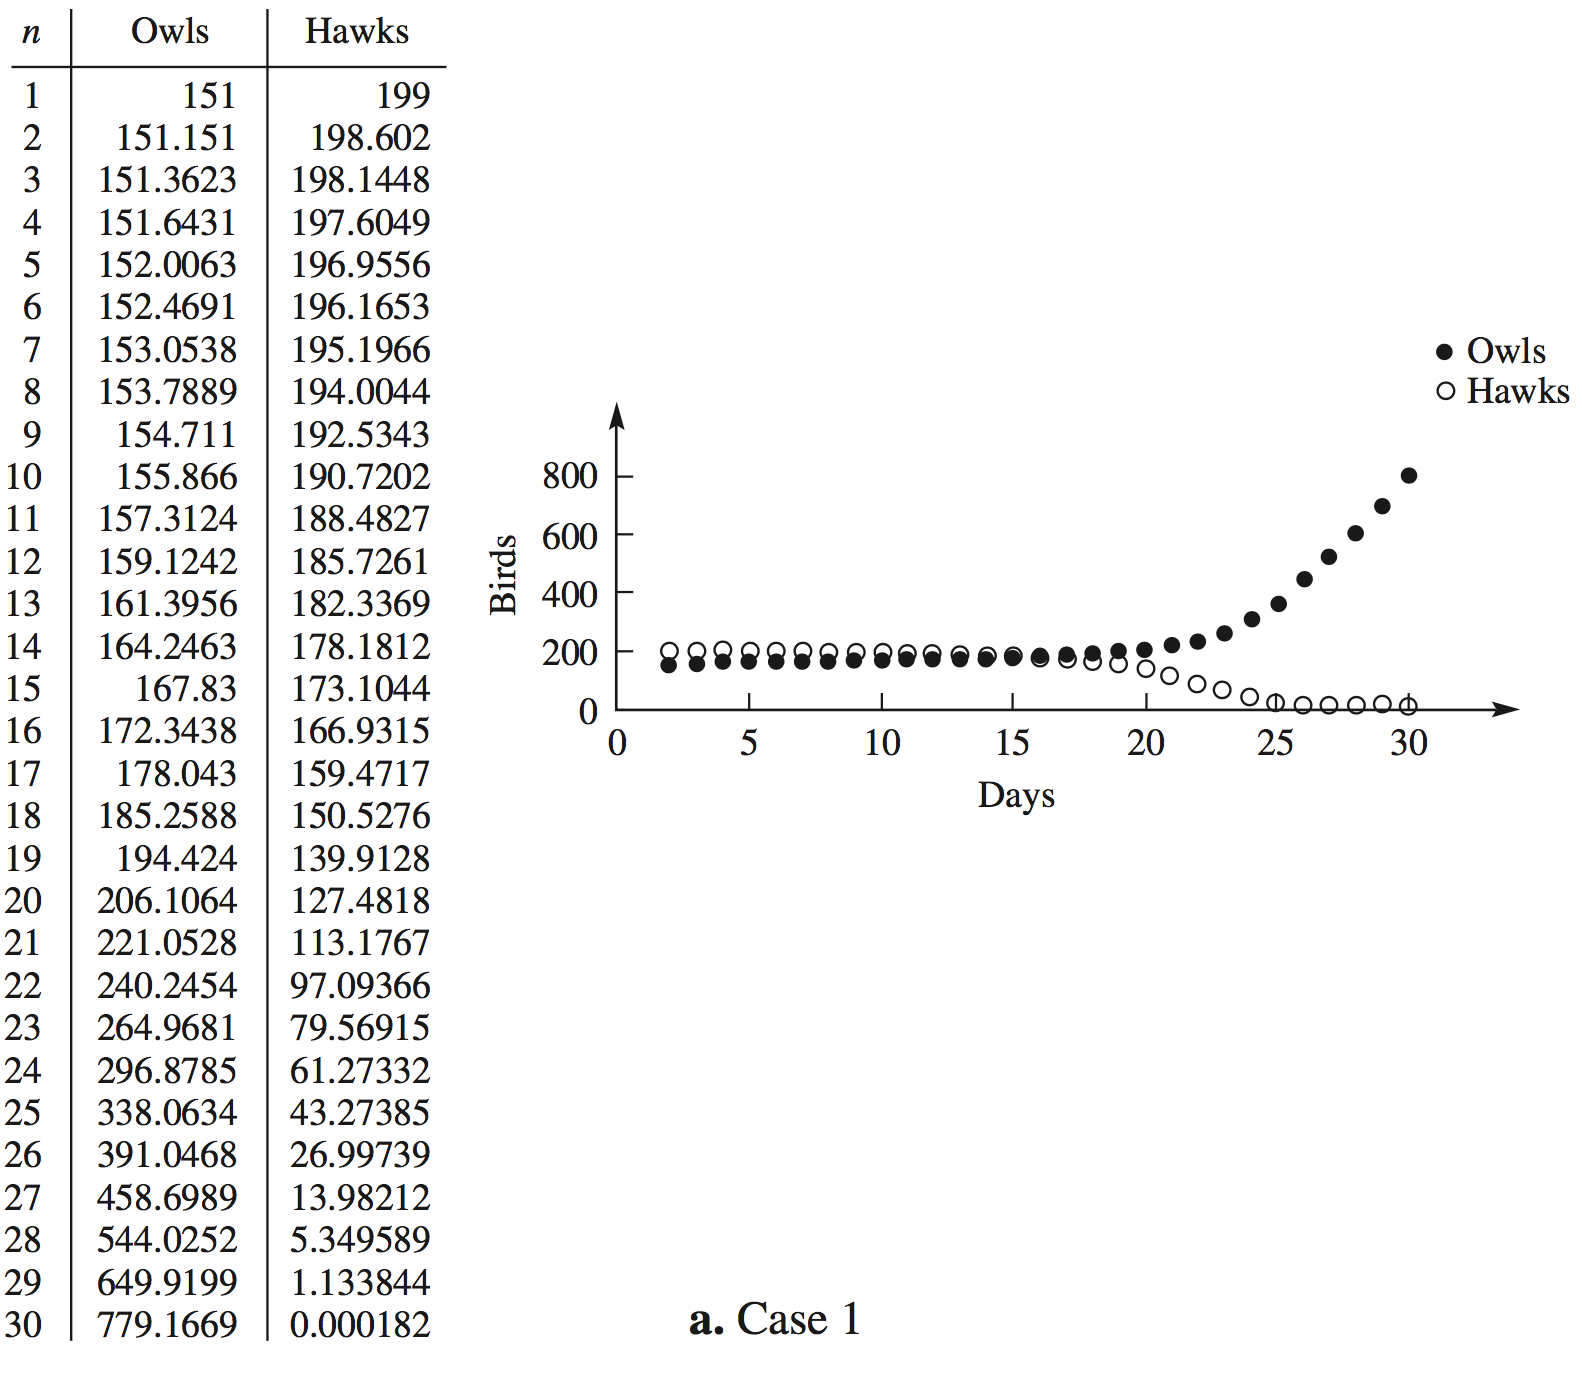
\includegraphics[height=.9\textheight{}]{owl-1.png}
  \end{center}  
\end{frame}

\begin{frame}{情况2}
  \begin{center}
    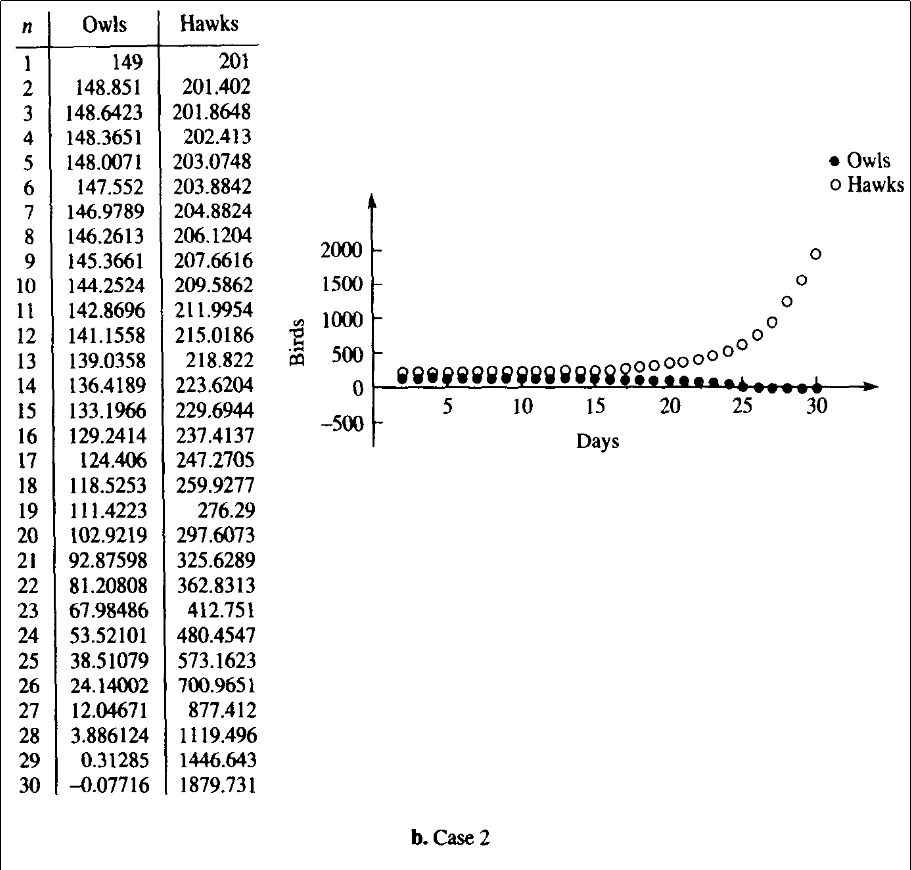
\includegraphics[height=.9\textheight{}]{owl-2.png}
  \end{center}  
\end{frame}

\begin{frame}{情况3}
  \begin{center}
    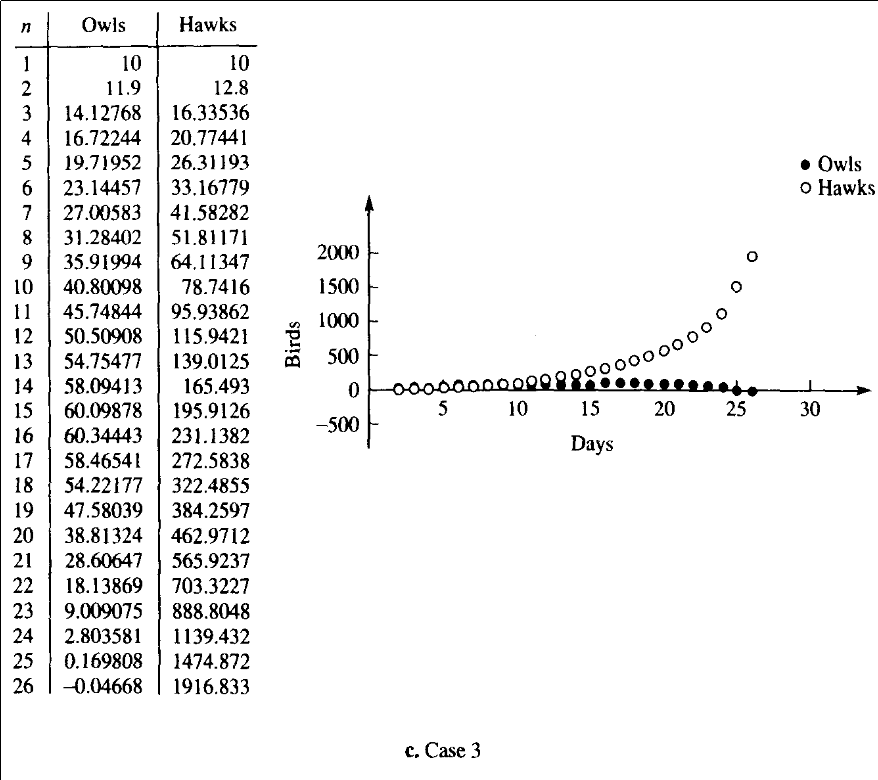
\includegraphics[height=.9\textheight{}]{owl-3.png}
  \end{center}  
\end{frame}

\begin{frame}{对初始条件的敏感性和长期行为}
  如果在栖息地安置350只猫头鹰和隼:

  \begin{enumerate}
  \item<1-> 如果150头为猫头鹰:猫头鹰和隼的数量不变(150、200)
  \item<2-> 如果149头或更少猫头鹰:猫头鹰将灭绝
  \item<3-> 如果151头或更多猫头鹰:隼将灭绝
  \item<4-> 该模型对初始条件极其敏感,平衡点不稳定。
  \end{enumerate}

\end{frame}

\begin{frame}{旅客趋势}
  \begin{center}
    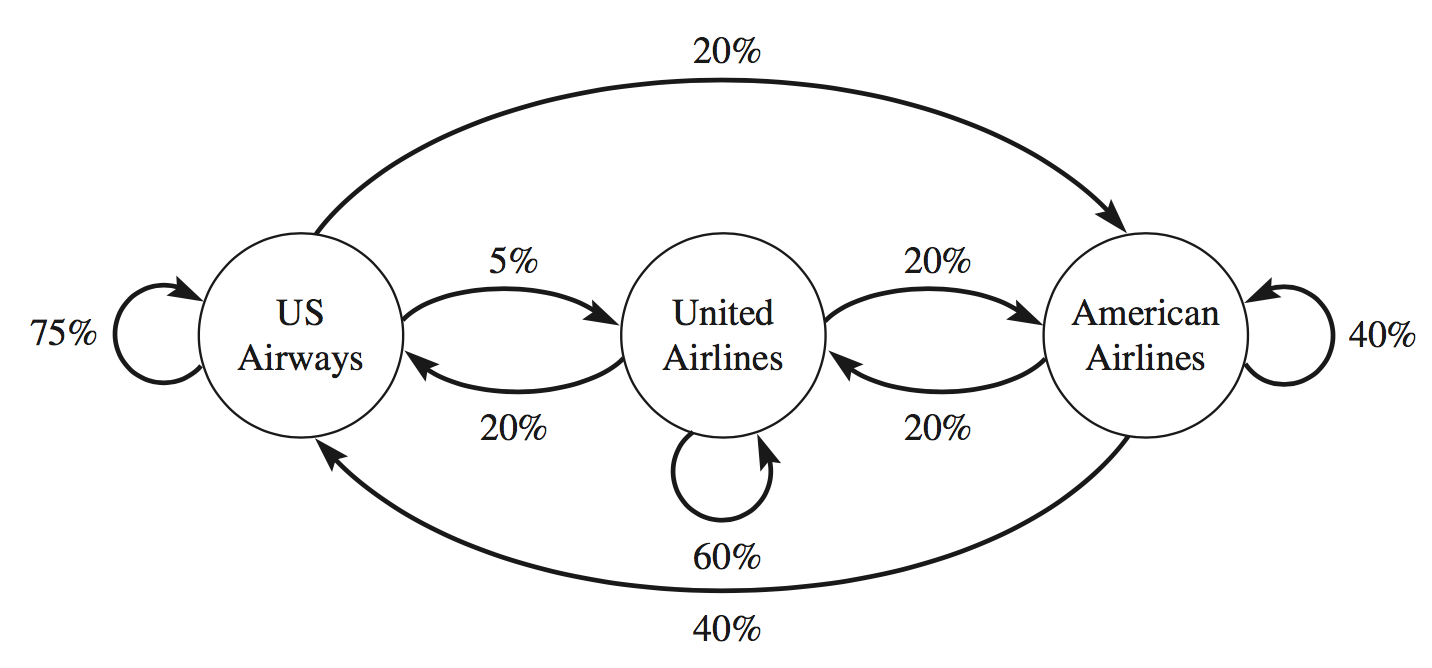
\includegraphics[width=.6\textwidth{}]{party.png}
  \end{center}  
  
  \begin{definition}
    $S_n = $ 第$n$个旅行周乘坐US Airways的旅客数\\
    $U_n = $ 第$n$个旅行周乘坐United Airlines的旅客数\\
    $A_n = $ 第$n$个旅行周乘坐American Airlines的旅客数
  \end{definition}
  
\end{frame}

\begin{frame}{差分方程组}
\[
S_{n+1}=0.75S_n+0.20U_n+0.40A_n
\]
\[
U_{n+1}=0.05S_n+0.60U_n+0.20A_n
\]
\[
A_{n+1}=0.20S_n+0.20U_n+0.40A_n
\]
平衡点$S_{n+1}=S_n=S$, $U_{n+1}=U_n=U$, $A_{n+1}=A_n=A$:
\[
-0.25S+0.20U+0.40A=0
\]
\[
0.05S-0.40U+0.20A=0
\]
\[
0.20S+0.20U-0.60A=0
\]
\end{frame}

\begin{frame}{平衡点分析}
$S:U:A = 2.2221:0.7777694:1$

\begin{center}
  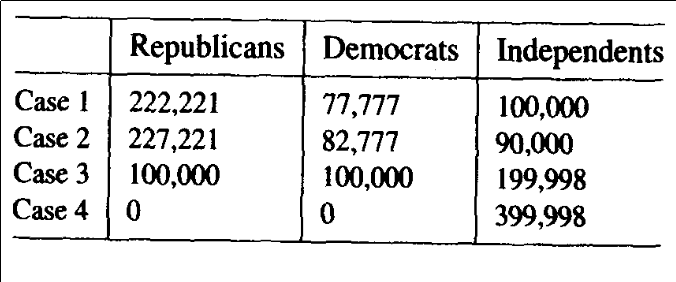
\includegraphics[width=.8\textwidth{}]{party-case.png}
\end{center}  
  
\end{frame}

\begin{frame}{情况1}
  \begin{center}
    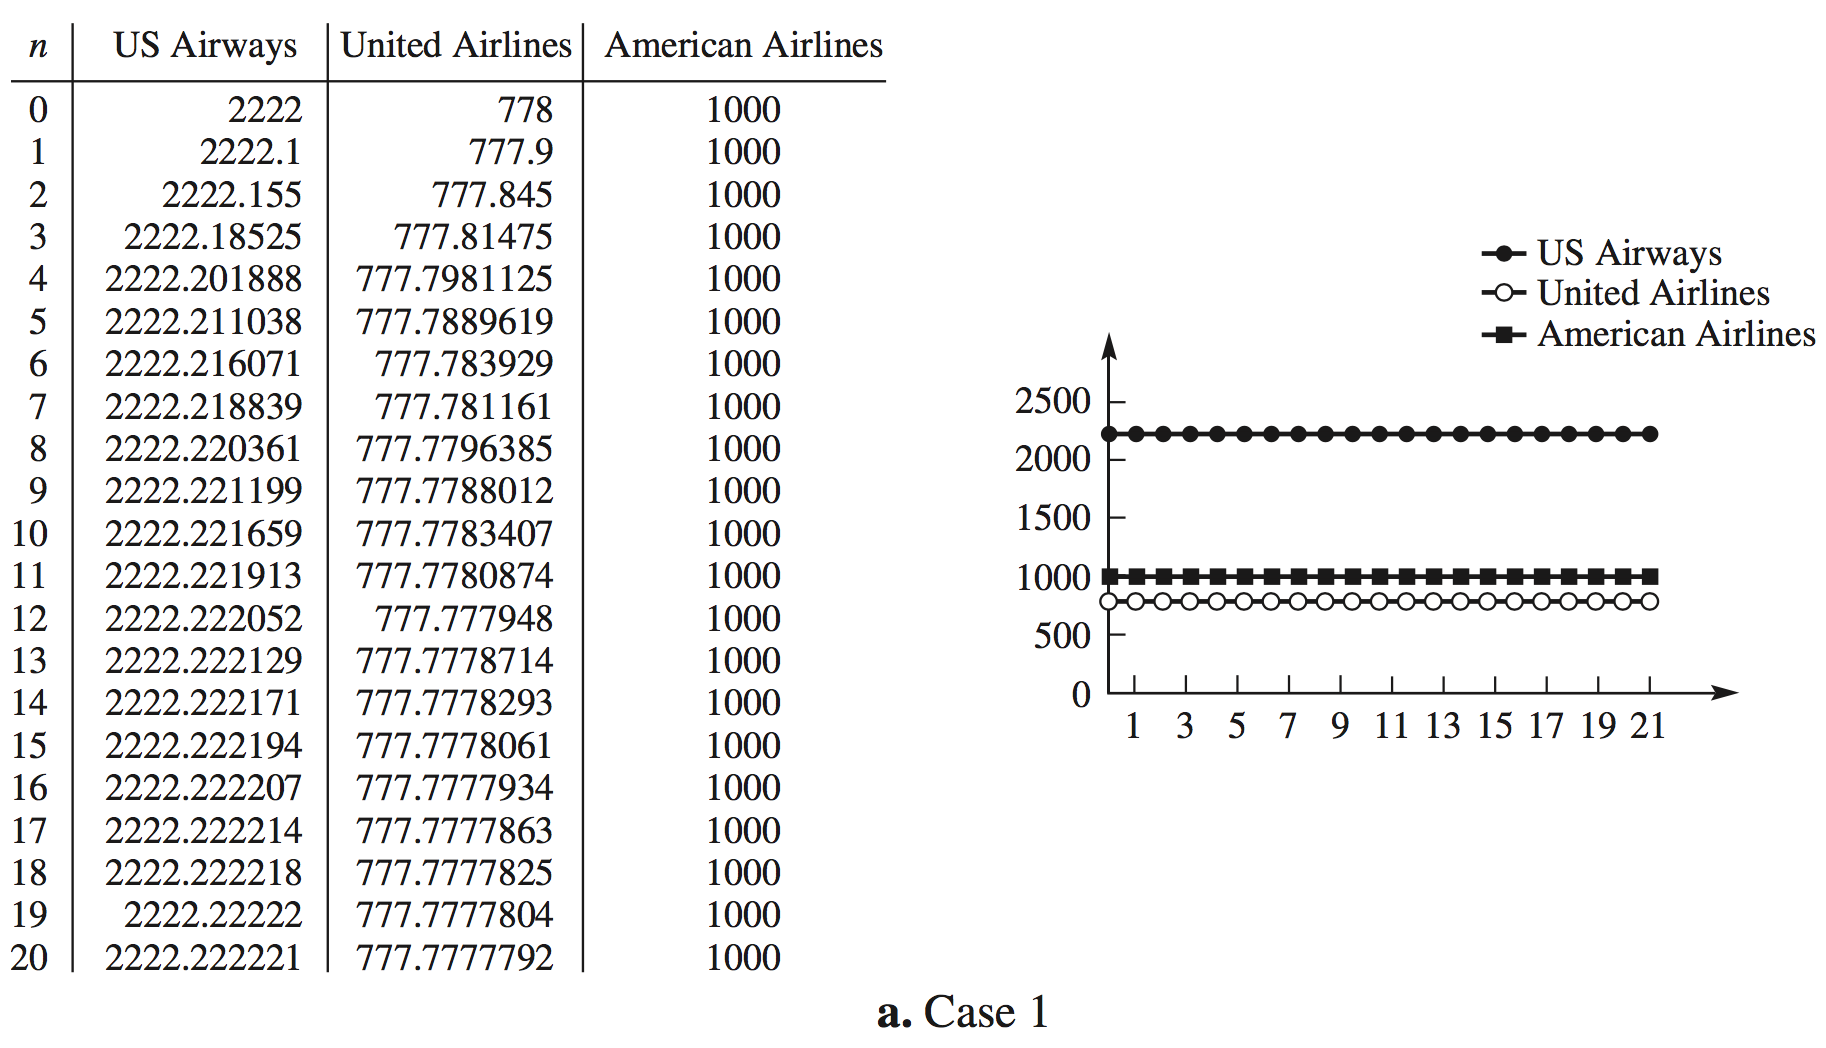
\includegraphics[width=.9\textwidth{}]{party-1.png}
  \end{center}  
\end{frame}

\begin{frame}{情况2}
  \begin{center}
    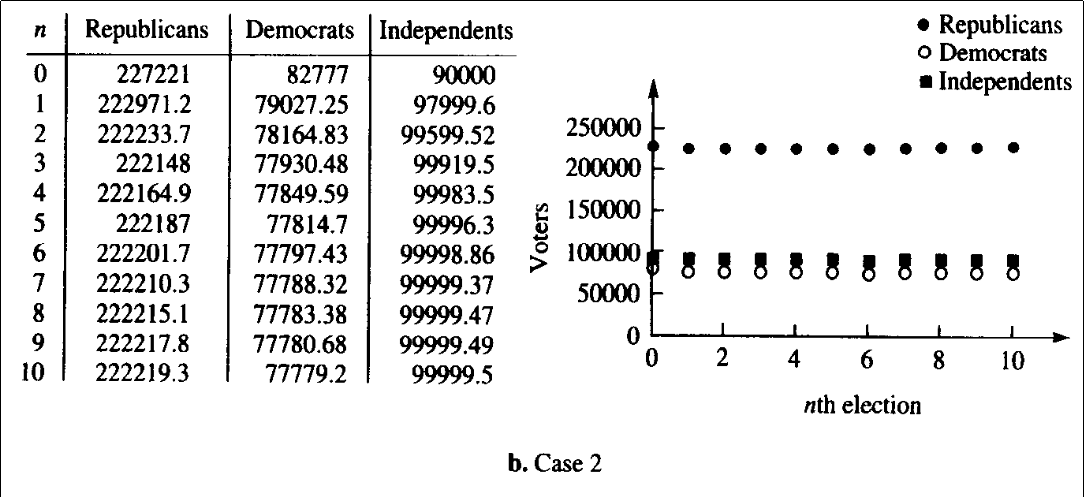
\includegraphics[width=.9\textwidth{}]{party-2.png}
  \end{center}  
\end{frame}

\begin{frame}{情况3}
  \begin{center}
    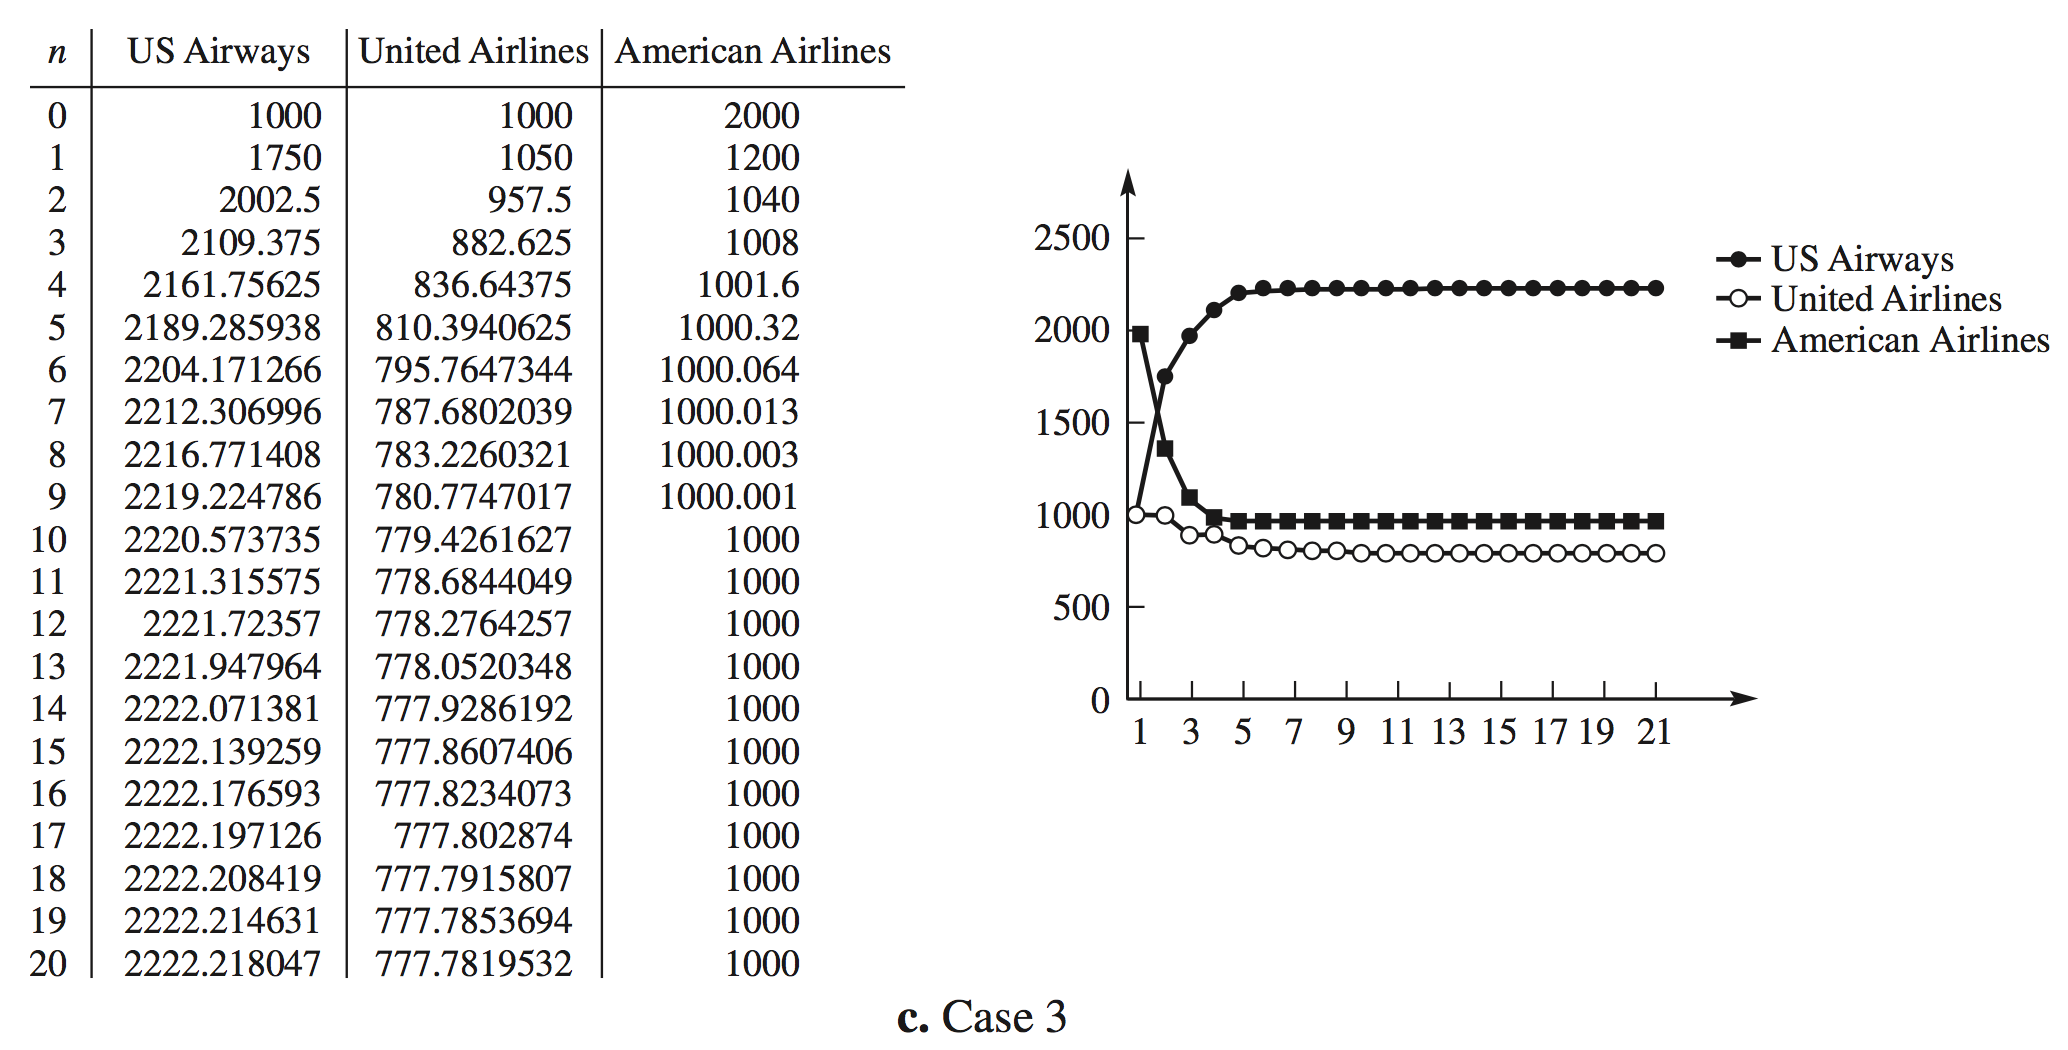
\includegraphics[width=.9\textwidth{}]{party-3.png}
  \end{center}  
\end{frame}

\begin{frame}{情况4}
  \begin{center}
    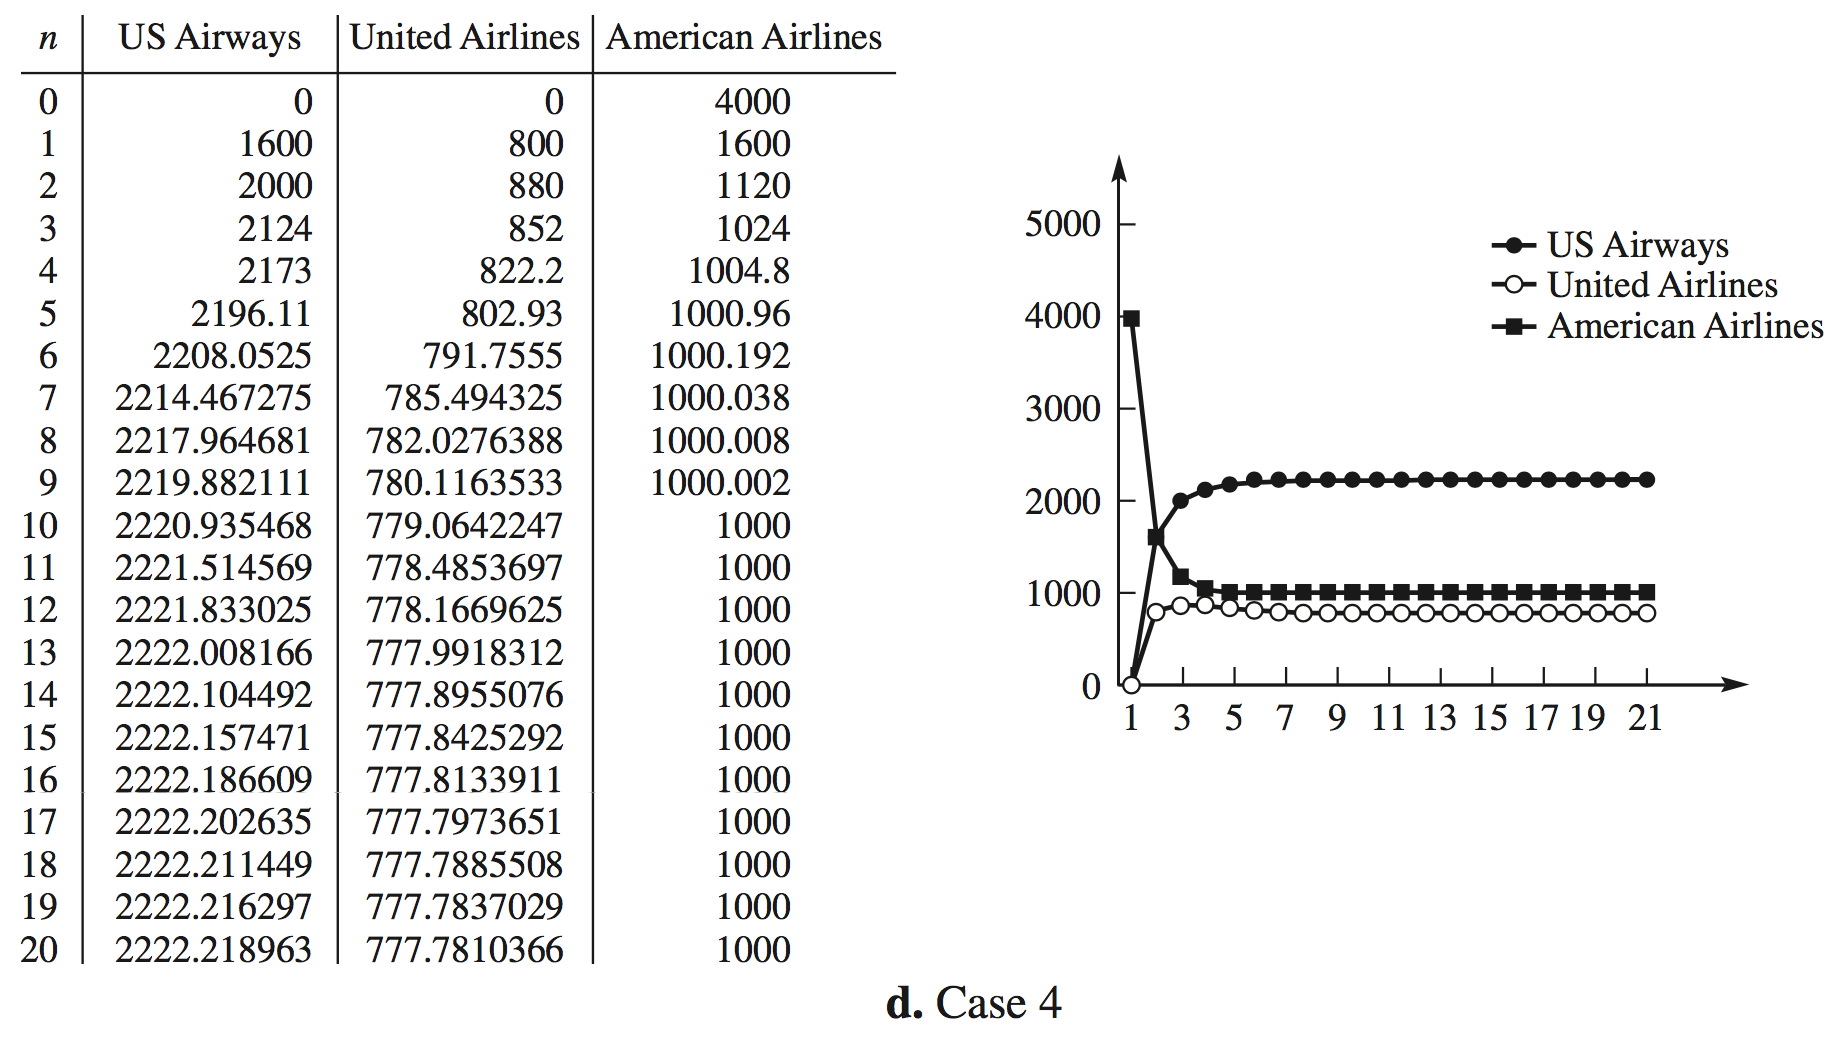
\includegraphics[width=.9\textwidth{}]{party-4.png}
  \end{center}  
\end{frame}

\begin{frame}{总结}
系统相当稳定,即使刚开始没有人坐US Airways和United Airlines的旅客数.
  
\end{frame}

\end{document}

%%% Local Variables: 
%%% TeX-master: t
%%% TeX-engine: xetex
%%% End: 
